\chapter{Konzeption und Aufbau des Prototyps}\label{sec:concept}
% In diesem Kapitel wird die Konzeption des Prototyps vorgestellt.
% % Sie enthält zunächst das methodische Vorgehen des Abschnitts, im Anschluss folgt eine Analyse der Spiele, die im Fokus der Arbeit stehen und die Frage aus welchen Aspekten diese in die Konzeption eingeflossen sind. Der Hauptteil der Konzeption umfassen das Game-Design des Prototyps.

Nachdem durch die Literaturrecherche in Kapitel \ref{sec:related-works} wichtige Funktionalitäten im Design identifiziert werden konnten und vergleichbare Spiele in Kapitel \ref{sec:analysis} auf ihr Game- und Rätseldesign analysiert wurden, kann aus den Ergebnissen \say{Connecting-Minds} nun vollständig konzipiert werden. \cite{krekhov_puzzles_2021} beschreibt eine Taxonomie für analoge und digitale Escape-Room Spiele, die ebenfalls in die Konzeption des Spiels hineinfließen.

Die Konzeption dieses Spiels folgt einem methodischen Vorgehen: Zunächst wird die übergeordnete Designvision und Zielsetzung erläutert. Anschließend dient das \ac{MDA}-Framework (vgl. \cite{hunicke_mda_2004}) als zentrales Analyse- und Strukturierungsmittel, um das Spielerlebnis gezielt zu gestalten. Auf Basis des \ac{MDA}-Frameworks werden die grundlegenden Spielmechaniken, Rollenverteilungen und dynamischen Abläufe beschrieben.


% [irgendwo muss noch Feedback aus dem vorangegangenen projekt erwähnt werden]
% \section{}

\section{Designziele und Zielgruppe}
\say{Connecting-Minds} verfolgt das Ziel, kooperative Kommunikation unter ungleichen Perspektiven in einem Escape-Room-ähnlichen Szenario zu verbessern. Dabei existieren zwei verschiedene Rollen - Player und Watcher - die gemeinsam die Rätsel lösen und Hindernisse der Spielwelt überwinden müssen. Die Wahrnehmung der Spielwelt und Handlungsmöglichkeiten ist in beiden Anwendungen unterschiedlich, gleichzeitig ergänzt sie sich aber. 

Das Genre des Spiels ist demnach ein kooperatives Adventure-Spiel.

Ziel ist es, durch asymmetrische Informationsverteilung eine Spannung zwischen Orientierung und Vertrauen aufzubauen und gleichzeitig den gemeinsamen Fortschritt in den Mittelpunkt zu stellen.

Die Zielgruppe bleibt dabei identisch zu der, die in der vorangegangenen Ausarbeitung im Modul \emph{Interaktionsdesign} entstanden ist.

Zunächst gibt es da den 19 Jahre alten Steve Works, der Medieninformatik-Student im ersten Semester ist. Er strebt nicht nur nach akademischen Erfolg, sondern auch nach sozialer Interaktion. Er plant gerne Spieleabende und Partys um Kontakte zu knüpfen und um den Spaß am Studieren zu betonen.

Uwe Kaufmann, 64 Jahre alt, ist ein erfahrenere Projektleiter und steht vor der Herausforderung ein neues Team zu formen. Sein Ziel ist es, durch Teambuilding und Motivation eine effektive Zusammenarbeit zu formen.

Anja Gayms, 31 Jahre alt, ist eine introvertierte Zahnarzthelferin und sucht in \say{Connecting-Minds} nach einer geistigen Herausforderung und einer Möglichkeit, ihre Freundschaften zu stärken.

Die 3 Personae sind in ihrer Gesamtheit in Anhang \ref{} verfügbar.


\section{Narratives und funktionales Grundgerüst}
% [Text nochmal kürzen]
Das Spiel basiert auf einem asymmetrischen Zwei-Rollen-Prinzip, bei dem zwei Spieler zwei unterschiedliche Rollen spielen. Sie müssen gemeinsam in der Spielwelt agieren. Die Spielwelt ist in verschiedene Räume gegliedert, welche modular aufgebaut sind. Durch das Zusammenarbeiten und das gemeinsame Lösen der Rätsel kann ein Spielfortschritt erzielt werden.
% Die beiden Rollen des Spiels werden Player und Watcher genannt. Der Player bewegt sich mit einer Isometrischen Perspektive durch die Spielwelt und kann die Ansicht bei Bedarf auch in die Egoperspektive wechseln. Er befindet sich dabei innerhalb der Spielwelt und interagiert von dort mit ihr.
% Der Watcher befindet sich ebenfalls in einer Isometrischen Ansicht, besitzt allerdings keinen eigenen Avatar in der Spielwelt. Er befindet sich außerhalb der Spielwelt, kann aber dennoch mit der Spielwelt interagieren. Der Watcher kann die Spielwelt in \ac{AR} vor sich platzieren um so um die Spielwelt herum zu gehen, oder sich einzelne Elemente näher anschauen.

Das Narrativ der Handlung und der Geschichte werden durch Textuelle Hinweise und Geschichten sowie dem Aufbau der Umgebung erzählt. 

% Funktional basiert das Spiel auf dem lösen von Rätseln und beseitigen von Hindernissen, die nur durch die Kombination beider Rollen lösbar sind.

Die Hintergrundgeschichte des Spiels ist folgende:

Der Protagonist der Handlung sollte in seinem Forschungsinstitut eine Simulation [Simulation zu was noch einbauen] ausprobieren. Allerdings kam es während der Simulation zu einer Anomalie, wodurch sich sein Sein aufgespalten hat. Übrig blieb sein physisches Ich, das in seinem Forschungsinstitut zurück blieb und sein abgespaltener Geist im Netz der Forschungseinrichtung verweilt. Sein aufgeteiltes Ich kann auf eine besondere Weise (vermutlich ausgelöst durch die Anomalie der Simulation) miteinander kommunizieren. Gemeinsam versuchen sie nun herauszufinden, wer für diese Anomalie verantwortlich ist und wie das physische Ich wieder mit seinem Geist zu einer Person zusammengefügt werden kann.

% Das Genre des Spiels ist demnach ein kooperatives Adventure-Spiel das in einem Low-Poly \ac{Sci-Fi}-Setting spielt.

% [Text zur Spielwelt, wo sich Schauplätze überall befinden ausdenken]
% Zunächst befinden sich die Spieler in einem alten Verlies
Die Spielwelt umfasst dabei zunächst ein altes Kellergewölbe der Forschungseinrichtung, in welcher der Körper des Players gebracht wurde, nachdem die Simulation schief lief. Des weiteren durchläuft der Player, mit seinem Watcher im Gepäck, die Forschungseinrichtung und sucht nach Hinweisen auf einen möglichen Antagonisten. Die Spielwelt wird erweitert durch Außenbereiche um die Forschungseinrichtung herum und geht weiter in die Privathäuser bzw. Wohnungen von beteiligten Personen.

\section{Spielkonzeption mithilfe des MDA-Frameworks}
Aus den bisherigen Forschungen zum Thema asymmetrischen kooperativen Spielen und Kommunikation geht hervor, dass die Spielerrollen des Spiels in ihren Funktionen und/ oder ihrer Ansichten eine Abhängigkeit von einender bestehen muss. Diese Abhängigkeit darf nicht zu groß sein, da sonst der Spielfluss gestört werden würde und Frust bei den Spielern entstehen könnte.

Die Analyse der artverwandten Spiele zeigten Inhalte und Funktionalitäten, die in ihrer Form integriert werden sollten, aber auch nicht zu eigenständig sein dürfen, wodurch ein kooperatives Verhalten gestört werden könnte.

Aus der \say{We were here}-Spielreihe geht hervor, dass die Rätselelemente so gestaltet werden müssen, dass diese für den anderen Mitspieler beschreibbar und verständlich erklärbar sind. Außerdem sollten die Anwendungen eine höhere Dynamik zwischen sich haben, wodurch eine engere Beziehung der Spielerfahrung und der Anwendungen entsteht. 

\say{Tiny Room Stories} zeigt wie einzelne Rätselelemente und freischalten von Hindernissen so zusammenhängen können, dass viele kleine Elemente zu einem großen Ziel führen können. Außerdem bietet es für die Steuerungsmechanik eine Inspirationsquelle. 

\say{The past within} zeigt, dass ein zu hohes Forderungslevel der einzelnen Anwendungen unvorteilhaft für die Förderung der Kommunikation ist. Es führt dazu, dass jeder Spieler auf seine Anwendung fixiert ist, aber seltener ein Gefühl dafür bekommt, wann er seinen Mitspieler benötigt und wann er selbständig Rätsel lösen kann. 

\say{Myrmidon} zeigt auf, wie die einzelnen Anwendungen abhängig zueinander sein können, allerdings fehlt es an einem ausgeglichenem Spielerlebnis. Die beiden Rollen sind so gestaltet, dass der Animator die Stop-Motion Puppe unterstützt und dadurch zu wenig für sich selbst spielt. 

Bei \say{Keep Talking and Nobody Explodes} ist es ähnlich wie bei \say{Myrmidon}. Die Spielerrolle der Experten unterstützt hierbei nur den Bombenentschärfer.

% Die Rückschlüsse sind folgende:

% \begin{itemize}
%     \item Aus der \say{We were here}-Spielreihe geht hervor, dass die Rätselelemente so gestaltet werden müssen, dass diese für den anderen Mitspieler beschreibbar und verständlich erklärbar ist.
%     \item Außer
%     % \item 
%     % \item 
%     % \item 
% \end{itemize}

% \subsection{Inhalte aus der Literaturrecherche}
% \subsection{Inhalte aus der Analyse der Spiele}
% \subsection{Inhalt aus der Taxonomie}

\subsection{Mechanics}
Die Mechanischen Elemente des Spiels werden in die zwei jeweiligen Spielerrollen (Player und Watcher) und allgemeingültigen Mechaniken aufgeteilt.

\paragraph{Player}
Der Player steuert entweder über die Maussteuerung (Point \& Click-System) oder über Touchinputs den Avatar in der Spielwelt. Über das Mausrad oder die Zoom-Touch Steuerung kann die Höhe der Kamera zum Avatar verändert werden. Außerdem kann er in der Ansicht zwischen der Standard isometrischen Perspektive und einer First-Person-Ansicht wechseln. Das \ac{UI} des Players besitzt eine Toolbar, über die der Avatar bestimmte Interaktionen mit den Weltgegenständen wie das Aufnehmen oder Platzieren vollführen kann. Außerdem kann der Player Gegenstände tragen und diese an den Watcher zurück schicken. Über die First-Person-Ansicht kann der Player ebenfalls Gegenstände platzieren.

Außerdem schaltet der Player neue Gegenstände in der Spielwelt frei, in dem er so nah an sie herangeht, dass er mit ihnen interagieren kann.

\paragraph{Watcher}
Der Watcher hat in seiner \ac{AR}-Anwendung die Spielwelt vor sich platziert und kann im physischen Raum um die Spielwelt herumgehen und auch in die Spielwelt hinein, um sich die Welt genauer anzusehen. Seine Aufgaben liegen darin, eine Übersicht über die Spielwelt und alle gesammelten bzw. platzierten Gegenstände zu bekommen. Er kann alle interagierbaren Gegenstände, die entdeckt und platziert wurden von der Spielwelt entfernen. Die Gegenstände gehen danach wieder in das Inventar über, auf welches nur er Zugriff hat. Er kann bestimmte Gegenstände in der Spielwelt über einen Touch-Input platzieren oder andere Gegenstände an den Player schicken, welche der Player dann trägt. 

Im weiteren Verlauf des Spiels kann der Watcher Gegenstände nicht nur platzieren oder entfernen, sondern auch in der Größe skallieren oder drehen.

\paragraph{Weltregeln}
Leichte Gegenstände können vom Player getragen und aufgenommen werden. Diese Gegenstände kann der Player in der Spielwelt über die Interaktions-Leiste oder in der First-Person platzieren. 

Schwere Gegenstände können nur vom Watcher platziert oder skaliert werden. Der Player kann jedoch über seine Interaktionen mit ihnen interagieren. Beide Arten von Gegenständen können, sobald sie entdeckt und in der Spielwelt platziert wurden, vom Watcher wieder entfernt werden.

Es existieren zudem Hinweise in Schrift- und Bildform, welche vom Player entdeckt und an den Watcher gesendet werden können. Sie gelten als Ergänzung zum Environmental Rätseldesign.

\subsection{Dynamics}
Die aus den Mechaniken folgenden Dynamiken beziehen sich auf die Asymmetrie in der Perspektive und den Informationen, die beide Spielerrollen haben und erhalten. Außerdem entsteht dadurch eine Kombination aus den gegebenen Informationen, um daraus die richtigen Ansätze für Lösungen zu finden. 
Es entsteht eine Kombination und Koordination der Fähigkeiten der beiden Rollen, durch welche erst das Lösen der Hindernisse ermöglicht wird.

Durch die AR-Anwendung des Watchers entsteht eine neue räumliche Orientierung, da die Spielwelt in die physische Welt eingebettet wird.


\subsection{Aesthetics}
Die durch das Spiel angesprochenen ästhetischen Eigenschaften sind Challenge, Fellowship und Expression. Das Spiel soll logisches Denken, die Kommunikation und die Koordination der Spielteilnehmer anregen. Außerdem soll durch die enge Verknüpfung der Rollen eine enge Zusammenarbeit entstehen, durch welche ein Gemeinschaftsgefühl aufgebaut werden soll. Durch die Kommunikation sollen die Spieler auch sich selbst näher kennenlernen und herausfinden wie man mit sich selbst am besten umgeht.

Untergeordnet steht das Narrativ des Spiels als Stütze für die Sinnhaftigkeit der Herausforderungen, die bewältigt werden müssen.


\section{Spielabläufe}
Die Spielabläufe des Spiels werden in zwei unterschiedliche Abschnitte unterteilt. Es gibt einen übergeordneten Ablauf für das gesamte Spiel und einen für jeden einzelnen Abschnitt.

\subsection{Ablauf des Spiels}
\begin{figure}[ht]
\centering
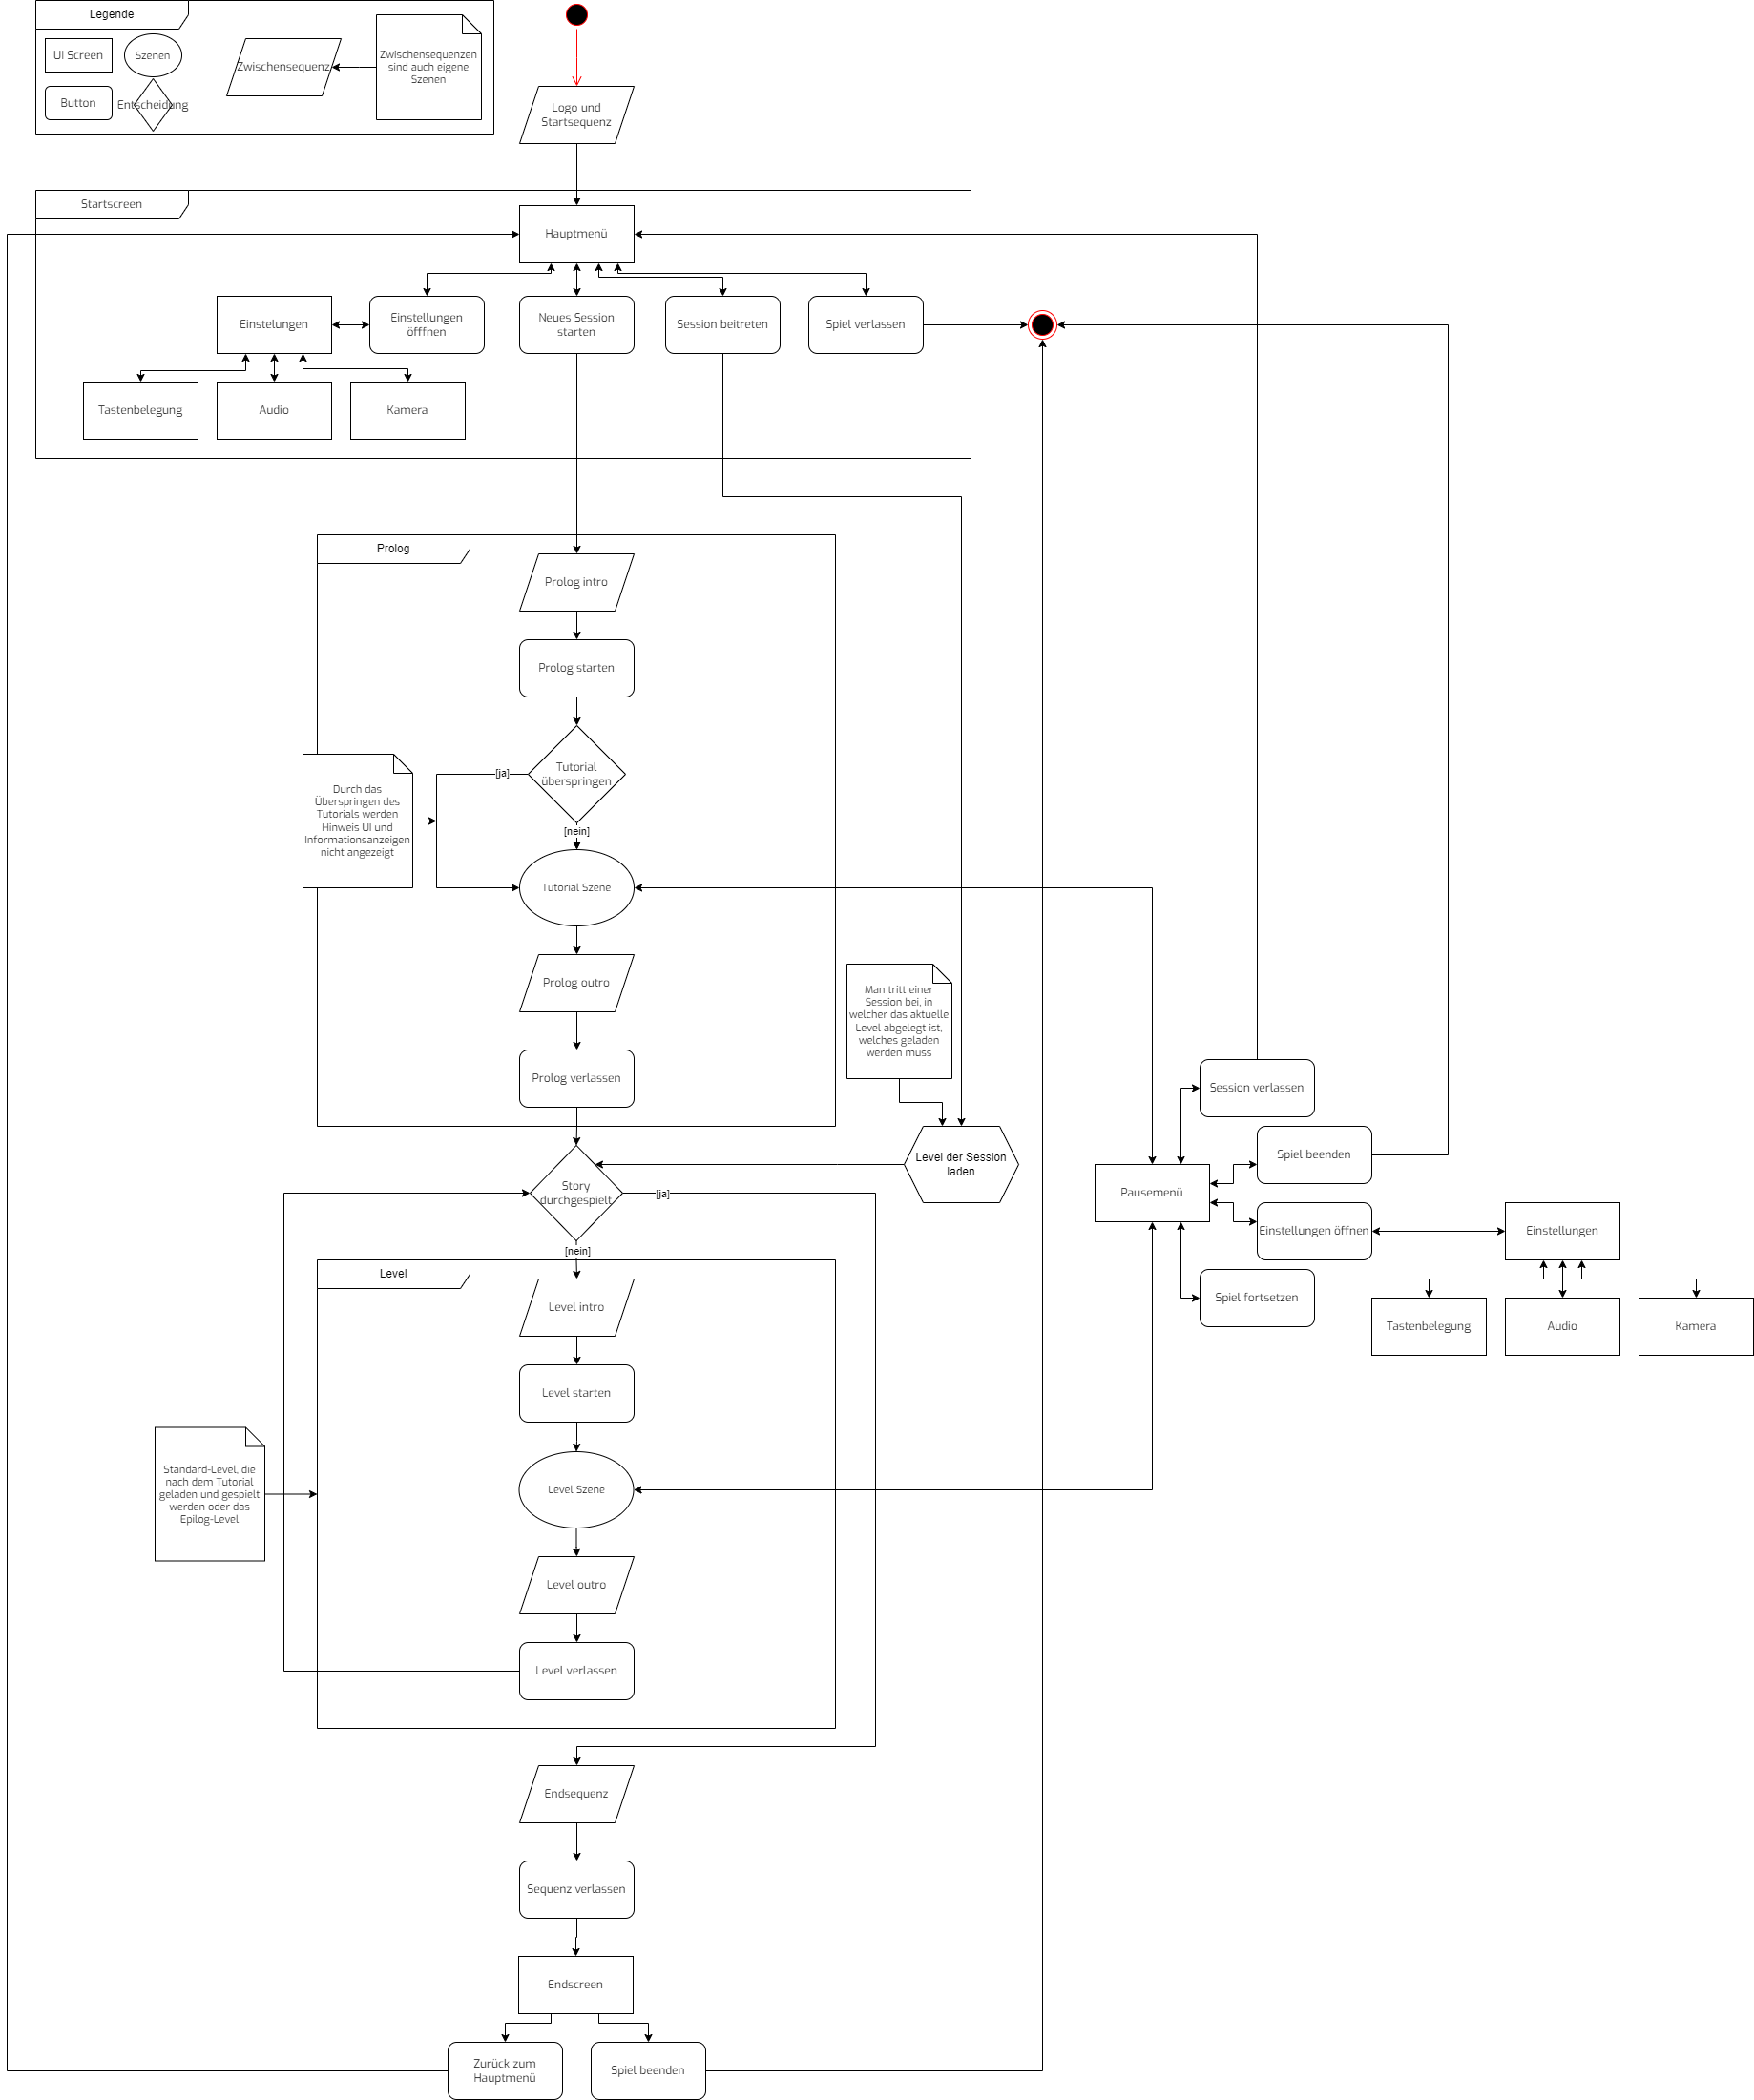
\includegraphics[width=1\linewidth]{content/pictures/GameLoop-Player.drawio.png}
\caption{Aktivitätsdiagramm des gesamten Spiels aus Player Sicht, (Quelle: eigene Darstellung), (in groß im Anhang \ref{})}
\label{fig:game-loop-player}
\end{figure}

\begin{figure}[ht]
\centering
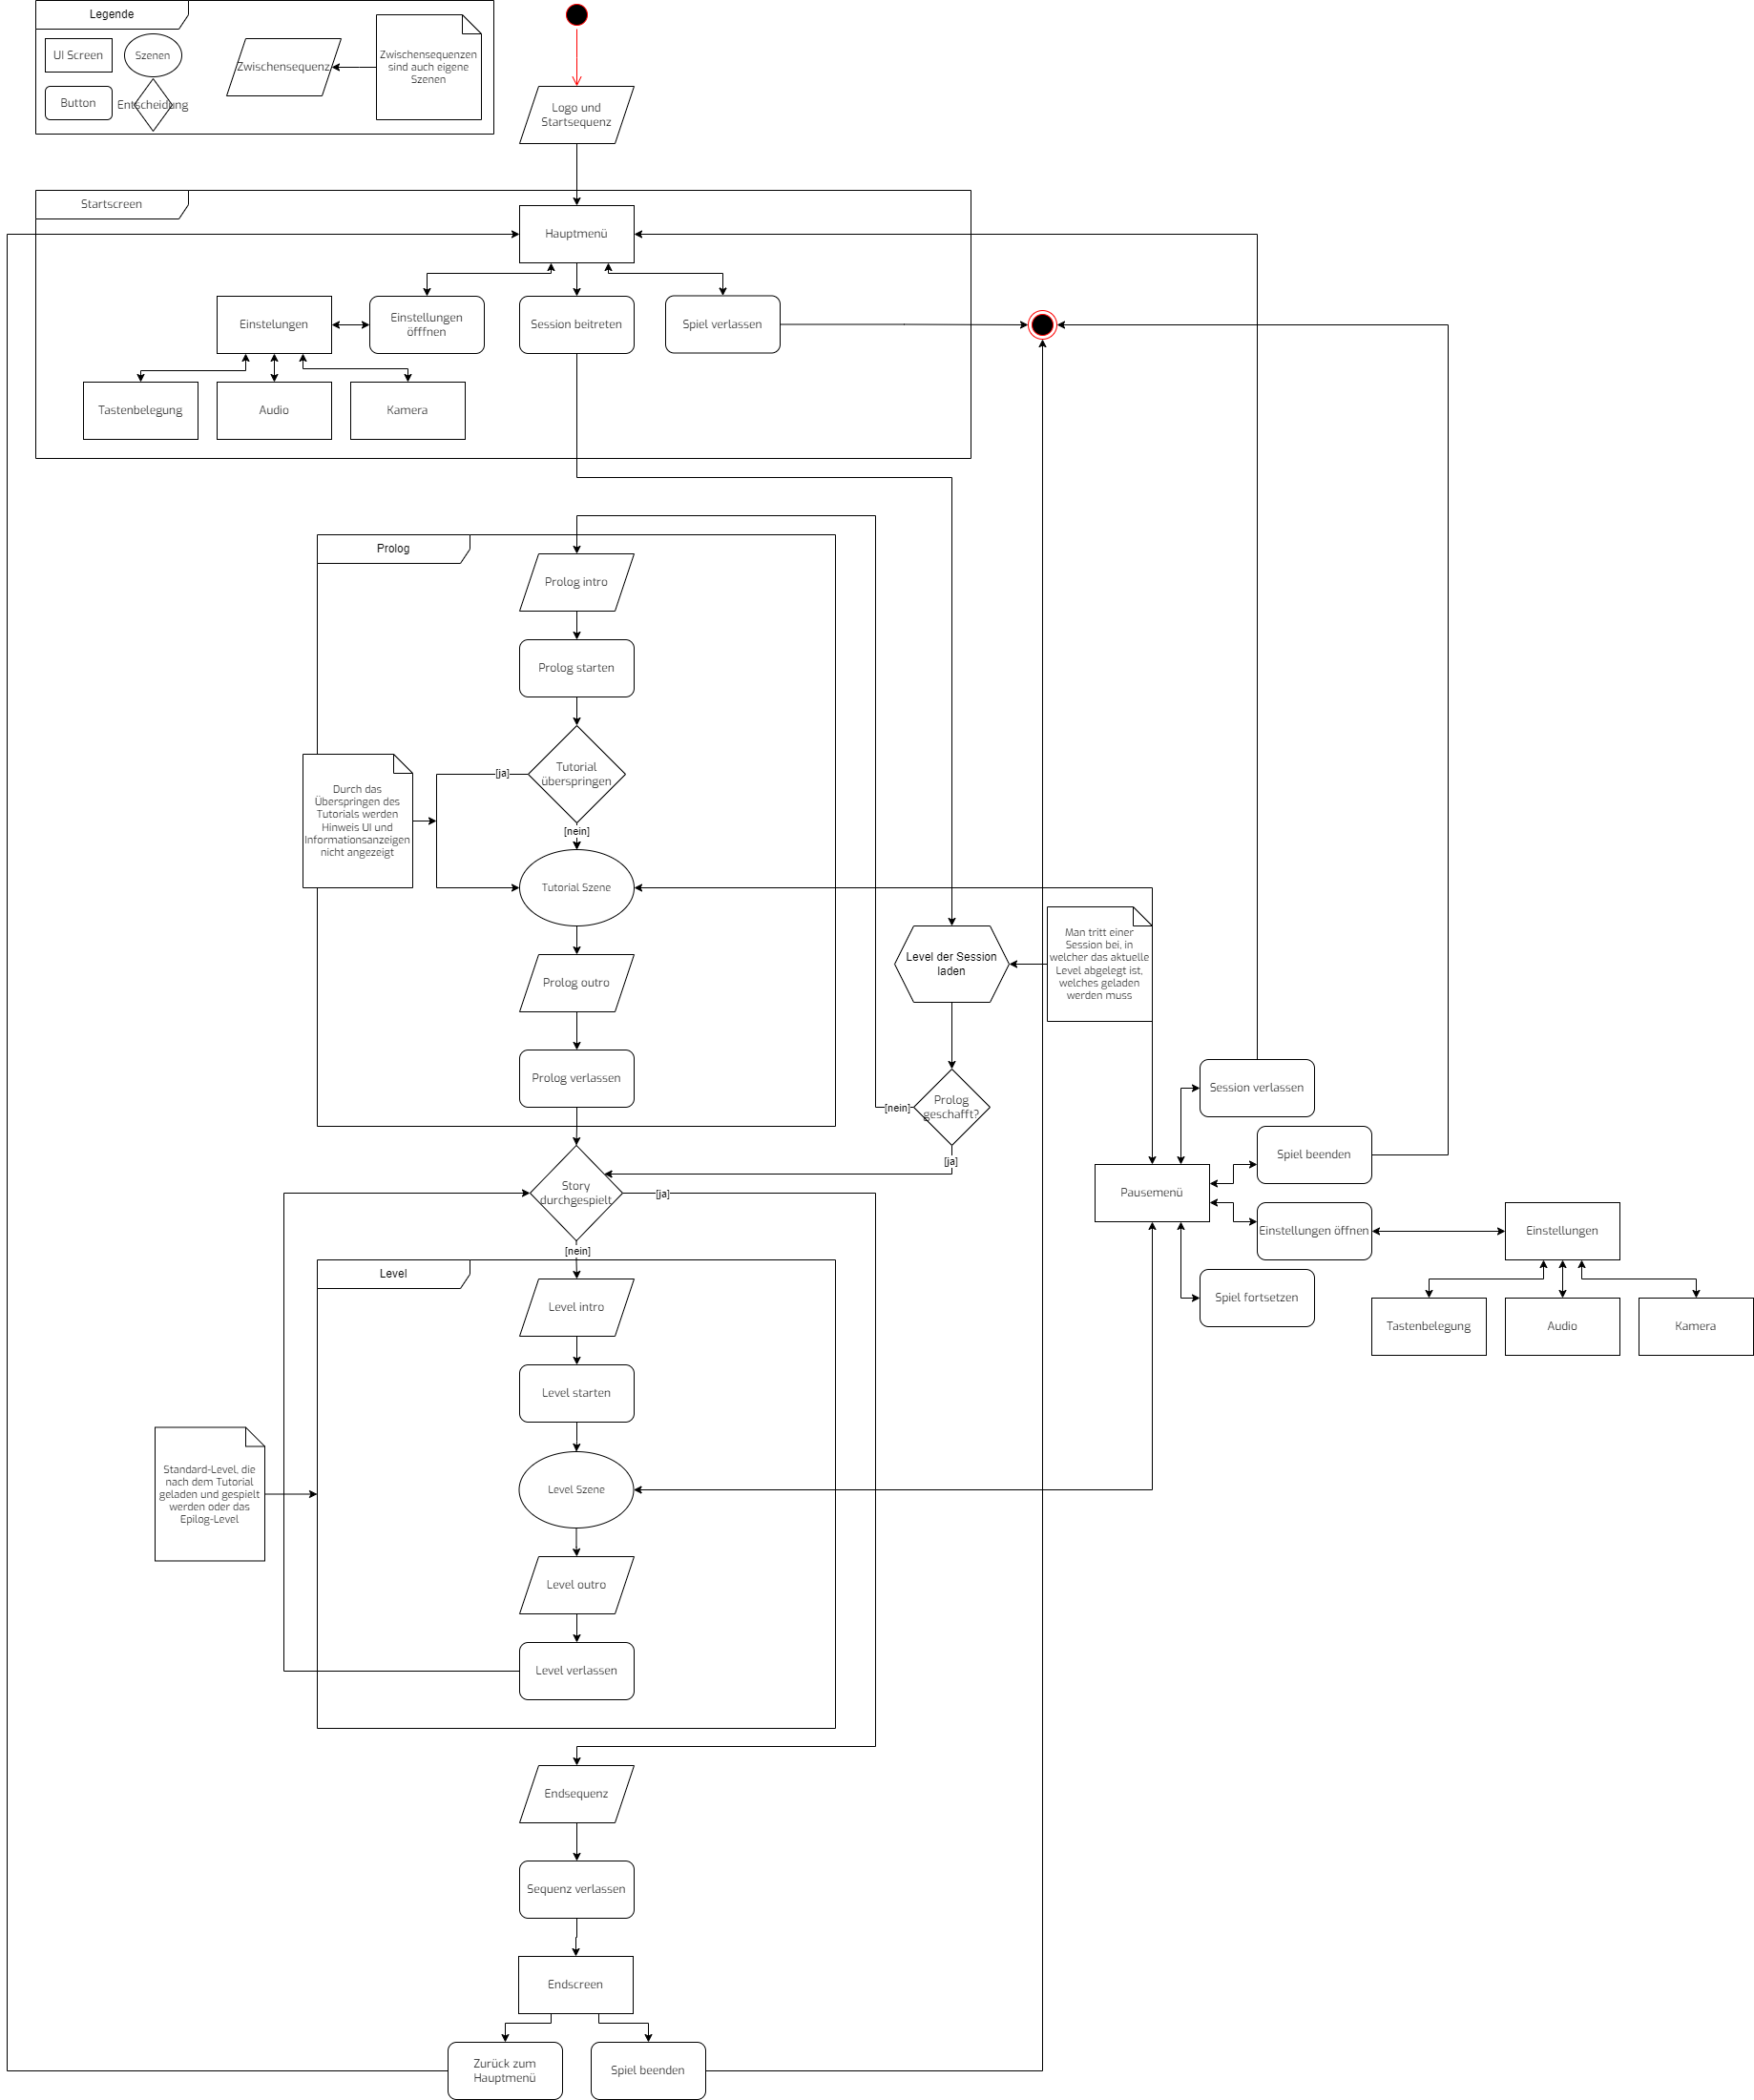
\includegraphics[width=1\linewidth]{content/pictures/GameLoop-Watcher.drawio.png}
\caption{Aktivitätsdiagramm des gesamten Spiels aus Watcher Sicht, (Quelle: eigene Darstellung), (in groß im Anhang \ref{})}
\label{fig:game-loop-watcher}
\end{figure}

Die Abläufe des Spiels sind bei den Anwendungen des Watchers und Players nahezu identisch. Es gibt allerdings einen Unterschied. Dieser wird in folgenden Beschreibung der Abläufe erklärt.
Abbildung \ref{fig:game-loop-player} zeigt das Aktivitätsdiagramm der Player-Anwendung. Sobald das Spiel geladen hat, öffnet sich das Startmenü über das der Player in die Einstellungen gehen, eine neue Session starten, einer existierenden Session beitreten oder das Spiel wieder beenden kann. Über die Einstellungen kann der Player die Tasten bzw. Touchbelegung einstellen, sowie Audio und Kameraeinstellungen ändern. Sobald der Player eine neue Session startet, öffnet sich die Prolog-Szene in der es ein kleines Tutorial zu den Regeln des Spiels und den Steuerungen gibt. 

Über die Tutorial-Inhalte erfährt der Spieler Informationen zu Interaktionsmöglichkeiten mit Gegenständen in der Welt. Sobald sich der Avatar des Players nahe an Gegenstände bewegt, die ein Tooltip haben, kann der Player über eine Leiste mit Interaktionen im UI mit den Gegenständen interagieren. Darunter fällt z. B. das bestätigen einer Taste bei einem Computer oder aber das Aufnehmen und Tragen von Gegenständen.

Es gibt für das Tutorial die Option erklärende Inhalte zu überspringen, da es sein kann, dass der Spieler das Spiel bereits einmal gespielt hat und die Inhalte nicht erneut lesen muss. Innerhalb der Spielszene kann der Player in ein Pausenmenü schalten, worüber er Einstellungen ändern, das Spiel beenden oder die Session verlassen kann. Außerdem kann er das Spiel auch wieder fortsetzen und weiterspielen. Verlässt der Spieler die Session, so lädt erneut der Startbildschirm und kann entweder der verlassenen Session neu beitreten oder eine neue Session starten.

Nach Abschließen des Tutorials wird die nächste Szene geladen, welche in der bestehenden Session gespeichert wird. Sobald der Player nun die Session verlässt und später erneut beitritt so lädt die Szene des abgespeicherten Levels. Dieser Kreislauf endet erst, sobald der letzte Spielabschnitt erreicht und die Geschichte beendet wurde. Über den Endscreen gelangt der Player erneut zum Hauptmenü, worüber eine neue Session gestartet werden kann. Das Beitreten der Session des beendeten Spiels führt dazu, dass der Player wieder im Endscreen landet und zurück ins Hauptmenü gelangt oder das Spiel beenden kann.

Bei der Anwendung des Watchers gibt es einen Unterschied zu der des Players. In Abbildung \ref{fig:game-loop-watcher} ist zu sehen, dass der Watcher nach Laden und Starten des Spiels keine Session starten sondern lediglich ein Spieler beitreten kann. Der Watcher ist so konzipiert, dass er nicht der aktive Teilnehmer, sondern ein unterstützender Teilnehmer des Spiels ist. Außerdem erhält der Watcher im Prolog für seine Aufgaben und seine \ac{UI}s entsprechende Informationen. Er erhält Informationen darüber, dass er über das Menü \say{Platzieren} Gegenstände in die Spielwelt platzieren kann und diese über den angezeigten Tooltip der Gegenstände auch wieder entfernen kann. Außerdem kann er über das Menü \say{Preview} Gegenstände an den Player senden, welche dieser trägt. Das gilt für jede Gegenstände die der Player trägt. Findet er einen Gegenstand und trägt ihn, so kann der Watcher ihn ebenfalls entfernen. Entdeckte Gegenstände werden wie platzierte Gegenstände in der Welt angezeigt.

Der restliche Spielablauf des Watchers ist identisch zu dem des Players.

\subsection{Ablauf des Levels}
Wie beim Ablauf des Spiels gibt es auch beim Levelablauf zwischen dem Player und Watcher kleine Unterscheidungen, die in der folgenden Erklärung aufgezeigt werden.

\subsection{Ablauf der Spielszene}
\begin{figure}[ht]
\centering
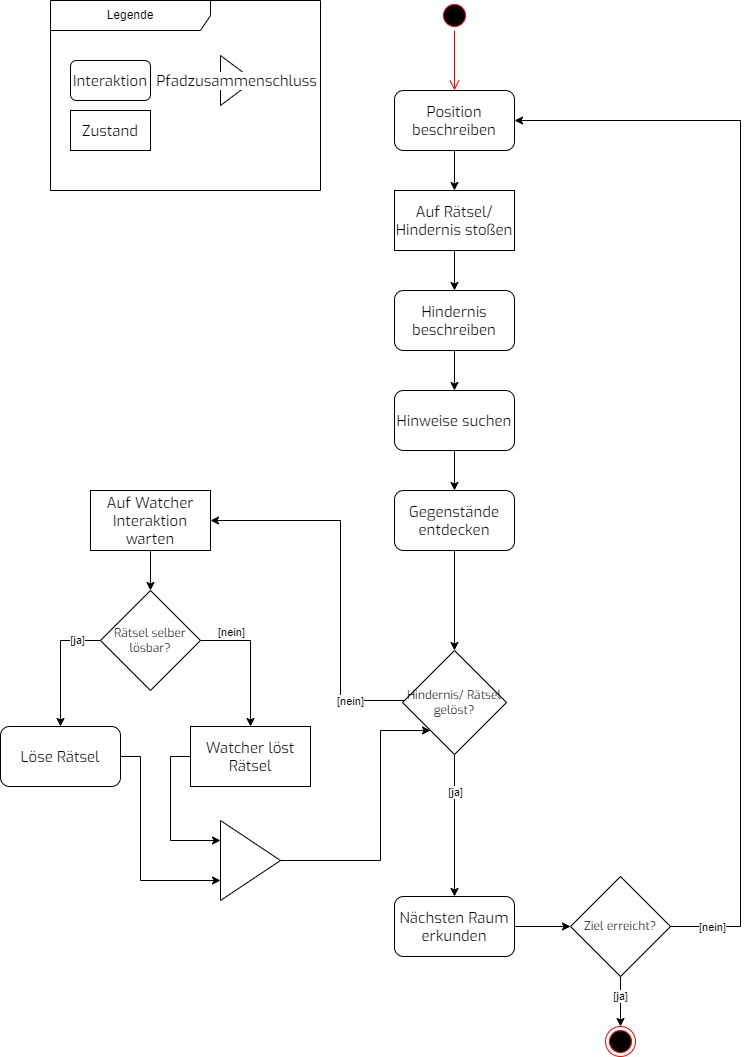
\includegraphics[width=1\linewidth]{content/pictures/LevelLoop-Player.drawio.png}
\caption{Aktivitätsdiagramm des Levels aus Player Sicht, (Quelle: eigene Darstellung)}
\label{fig:level-loop-player}
\end{figure}

\begin{figure}[ht]
\centering
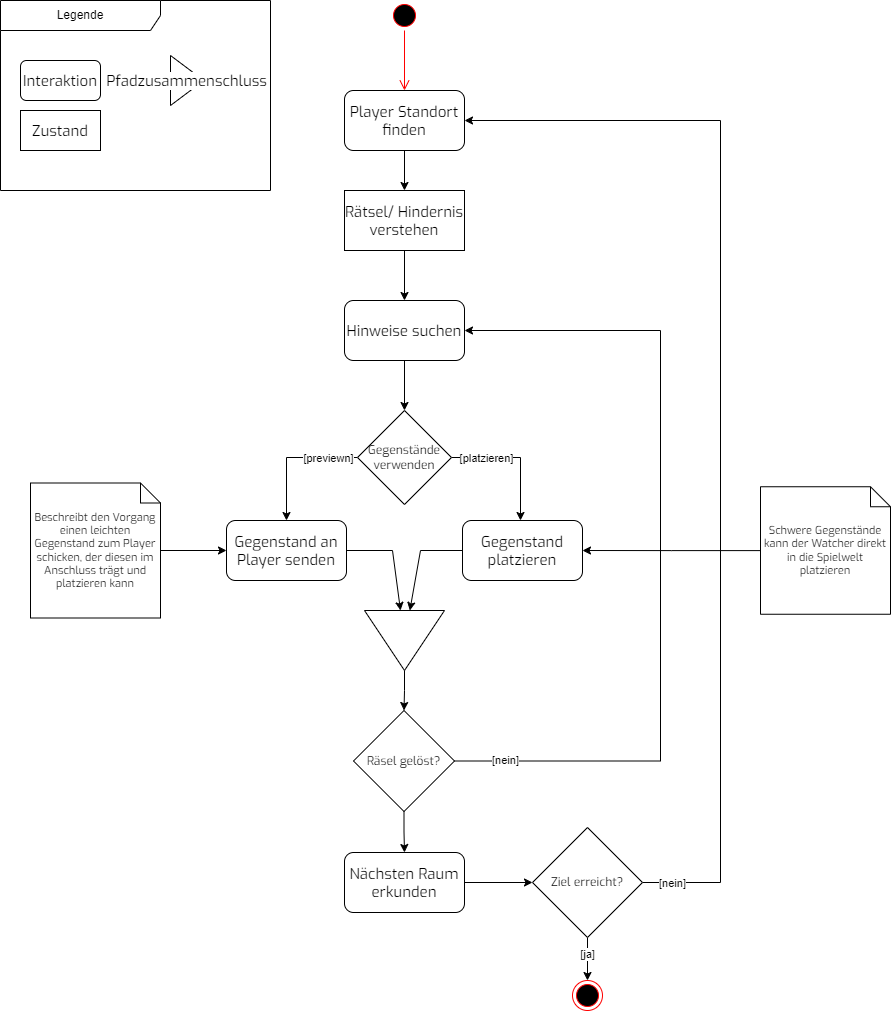
\includegraphics[width=1\linewidth]{content/pictures/LevelLoop-Watcher.drawio.png}
\caption{Aktivitätsdiagramm des Levels aus Watcher Sicht, (Quelle: eigene Darstellung)}
\label{fig:level-loop-watcher}
\end{figure}

Abbildung \ref{fig:level-loop-player} zeigt das Aktivitätsdiagramm des Players innerhalb der Spielszene. Sobald die Szene geladen hat, befindet sicher der Avatar des Spielers irgendwo in der Spielwelt. Da der Watcher den Avatar des Players nicht sehen kann, muss der Player seine Position beschreiben. Entweder nachdem der Player seine Position beschrieben hat oder währenddessen kann er sich in der Welt umsehen und stößt auf erste Rätsel oder Hindernisse. Ist dem so, so muss er seinem Watcher beschreiben um was für ein Rätsel oder Hindernis es sich handelt. In der Spielwelt befinden sich passende Lösungsgegenstände zu den Rätseln, die vom Player entdeckt werden können. Haben der Player und der Watcher das Rätsel gelöst so kann es sein, dass der Player darauf warten muss, dass der Watcher die richtigen Gegenstände in die Spielwelt platziert, damit sie weiter voran kommen oder aber der Watcher muss dem Player die richtigen Gegenstände schicken, damit dieser die Gegenstände an entsprechende Slots oder Stellen platzieren muss. Sobald ein Rätsel gelöst oder Hindernis beseitigt wurde, kommen sie weiter in der Spielwelt voran und müssen die nächsten Räume untersuchen. 

Beim Watcher, dessen Aktivitätsdiagramm in Abbildung \ref{fig:level-loop-watcher} zu sehen ist, verhält es sich ein wenig anders als beim Player. Der Watcher muss zunächst den Standort des Players durch seine Beschreibungen lokalisieren. Während der Lokalisierung und im Anschluss darauf kann er Hindernisse oder Rätsel erkennen und diese dem Player Beschreiben. Außerdem kann er sich bereits Gedanken zu Rätseln und Hindernissen machen, die der Player bereits entdeckt hat. Gemeinsam suchen sie getrennt nach Hinweisen und versuchen Lösungen zu finden. Das Lösen der Rätsel funktioniert aus der Sicht des Watchers ein wenig anders, da er dafür zuständig ist, die jeweilig richtigen Gegenstände zu platzieren und/ oder dem Player zu senden. Sobald alles Rätsel in Koordination gelöst wurden und neue Räume zugänglich sind, fängt der Ablauf von neuem an.

\section{Relation der Anwendungen}
In der bisherigen Konzeption wurde bislang nur über die verschiedenen Rollen gesprochen, aber nicht wie viele Nutzer pro Rolle es pro Session des Spiels sein können. In der Entstehung des Projekts in der vorangegangenen Ausarbeitung war geplant, dass es pro Session immer einen Player geben muss. Außerdem können es immer mehr als einen Watcher geben. Es sollte also diese Regel gälten: $1\ldots n$ \quad wobei $n \geq 1$. In einer Referenz-Bachelorarbeit wurde ein ähnlicher Prototyp konzipiert, bei der in der Auswertung das Feedback gegeben wurde, dass sich mehrere Teilnehmer in der Rolle der \say{Smartphone}-Nutzer (Navigator) nicht zielführend sind (vgl. \cite[S. 34]{lotz_konzeption_2021}). Aus diesem Grund und der Tatsache, dass die Rolle des Watchers eine ähnliche des Navigators ist, sollten pro Session jeweils ein Player mit einem Watcher gemeinsam spielen. Darüber hinaus erforschte die Arbeit von \cite[S. 197:22]{bautista_isaza_understanding_2024} den Einfluss der Gruppengrößen auf das Engagement und die Arbeitsbelastung in einem Handheld-\ac{MR} und \ac{VR} Szenario und kam zu dem Schluss, dass kleinere Gruppen der Effekt des Engagements größer ist. Daraus ergibt sich die Regel $1\ldots1$, durch welche ein Player und ein Watcher in einer Session zusammenspielen.
% \section{Levelablauf}

\section{Konzeption des Tutorials}
% [TODO: bei den Rätsel muss noch ein Bezug aif Pattern und so erfolgen]

Für diesen Prototyp wurde ein kleines Tutorial konzipiert, durch welchen der Watcher und der Spiele die grundlegenden Mechaniken und Funktionen des Spielkonzepts erlernen können. Aus dem Grund des Umfangs der Umsetzungen, wurden in den Probandentests die einzelnen Funktionen und Steuerungselemente erklärt, die in einer finalen Version im Spiel enthalten sein werden. Außerdem beinhalten die Konzepte der Rätsel bereits das überarbeitete Design nach dem Feedback aus den kommenden Probandentests.

% [Die gesamten Lernziele des Tutorials hier einbauen]
Folgende Lernziele wurden für das Tutorial konzipiert:
\paragraph{Watcher}
\begin{itemize}
    \item Steuerung in der Anwendung (Drag, Zoom, Yaw und Touch)
    \item Auffinden der richtigen Position, an der sich der Avatar des Players befindet 
    \item Identifizierung des Ziels, wohin er den Player navigieren muss
    \item Identifizierung von Hinweisen und Rätseln
    \item Platzieren von schweren Gegenständen
    \item Previewen von leichten Gegenständen
    \item Entfernen von platzierten Gegenständen
    \item Identifizierung von Unterschieden in der Spielwelt
\end{itemize}

\paragraph{Player}

\begin{itemize}
    \item Steuerung in der Anwendung (Drag, Zoom, Touch)
    \item Identifizierung und Beschreibung der Lokalität
    \item Identifizierung von Hinweisen und Rätseln
    \item Tragen von Objekten (Previewen)
    \item Interaktion mit interagierbaren Weltobjekten
    \item Entdecken von neuen schweren und leichten Gegenständen
\end{itemize}

Das Tutorial wurde in verschiedene Abschnitte unterteilt, welche sich in einzelne Räume gliedern. Die einzelnen Abschnitte mit ihren Lernzielen und ihre Räumen werden nun vorgestellt.
\subsection{Abschnitt 1: Der Start}
Zunächst werden die Lernziele dieses Abschnittes vorgestellt, aus welchen der Abschnitt konzeptionell gestaltet wird.

\paragraph{Lernaspekte und Konzeption dieses Abschnittes}
Der Watcher bekommt eine kleine Einführung in die genannten Steuerungsmechaniken seiner Anwendung. Daraus resultiert, dass er sich selbständig durch die Spielwelt navigieren kann. Die Kernaufgabe des Watchers ist es, die Bewegungen des Players nachverfolgen zu können, wofür er die Position des Players benötigt. Daher sollte die Spielwelt so gestaltet sein, dass eine Positionsbeschreibung des Players automatisch erfolgen muss. Dies geschieht durch unterschiedliche Startpositionen in der Spielwelt, welche vom Player beschrieben werden muss, wodurch der Watcher den richtigen Startort suchen muss. In Abbildung \ref{fig:sketch-starterrooms} wird eine kleine Sketchzeichnung zum Startgebiet gezeigt. 

\begin{figure}[ht]
\centering
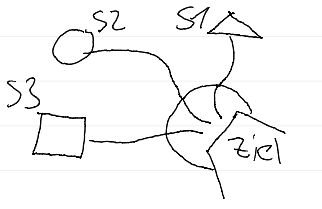
\includegraphics[width=1\linewidth]{content/pictures/Startplaces_Sketch.png}
\caption{Sketchzeichnung der Starträume (Quelle: eigene Darstellung)}
\label{fig:sketch-starterrooms}
\end{figure}

Der Watcher muss auch erkennen können, wohin sie gemeinsam gehen müssen. Daher muss die Spielwelt immer so eindeutig sein, dass es entweder ein oder mehrere eindeutige Ziele geben muss, wohin der Player gelotst werden muss. Für einen ersten Abschnitt ist es allerdings einfacher, wenn ein Ziel festgelegt wird, wohin alle Wege führen. In Abbildung \ref{fig:sketch-starterrooms} ist dieses klar im Sketch zu sehen. 

Die mit der Spielmechaniken einhergehenden Grundmechaniken und Aufgaben des Watchers müssen ebenfalls erlernt werden, darunter zählen das Platzieren, Previewen und Entfernen von Gegenständen. Das Platzieren von Gegenständen kann so initialisiert werden, dass der Watcher zu, Start des Spiels bereits einen Gegenstand wie eine Säule im Inventar hat, welche nun nur noch den Ort benötigt, wo sie platziert werden kann. Durch ein weiteres Hindernis und dem Erkennen, dass der Player einen Gegenstand benötigt den er in eine bestimmte Stelle platzieren muss, bekommt der Watcher die Aufforderung dem Player einen bereits existierenden Gegenstand (bspw. eine Fackel) zu schicken. Das Entfernen von Gegenständen kann so so initialisiert werden, dass der Player in der in der Sketchzeichnung eingezeichneten Ziel-Eingangshalle ist (vgl. Abbildung \ref{fig:sketch-starterrooms}) und dort eine Tür oder ähnlcihes zu einem weiteren Abschnitt öffnen muss. Es werden allerdings wieder die gleichen Gegenstände benötigt, die sie in den vorangegangenen Rätseln verwendet haben. Also müssen die in der Welt platzierten Gegenstände entfernt und erneut platziert werden.

% [Einfügen von unterschieden in der Spielwelt, erklärend aus Feedback vom vorangegangenen Projekt und hier eimbauen wie es in der Umsetzung aussehen kann]
Darüber hinaus lernt der Watcher die Spielkarte richtig zu deuten. Es gibt in der Darstellung der Spielwelt in der Player-Anwendung teilweise kleine Unterschiede zu der des Watchers. Dieser Aspekt soll zudem die Kommunikation fördern. Umgesetzt ist dieser Aspekt durch fehlende Türen in den Starträumen, in denen der Player zu Beginn des Spiels ist, und bei den Durchgängen zum Eingangsportal zum nächsten Abschnitt.

Analog zum Watcher, erhält der Player ebenfalls eine kleine Einweisung in die Steuerungsmechaniken der Anwendung. im Allgemeinen sind in der Anwendung des Players Rätsel und Hindernisse eingebaut, partiell allerdings in der Anwendung des Watchers. Aus diesem Grund muss der Player Rätsel/ Hindernisse und Hinweise identifizieren und verwenden können. Um einen ersten Anhaltspunkt für den Start zu erhalten, sollte in den jeweiligen Starträumen des Players eine kleine Notiz eingebaut werden, welche einen Hinweis auf die Einführung der Mechaniken des Watchers und das Lösen des ersten Hindernisses geben.
\begin{figure}[ht]
\centering
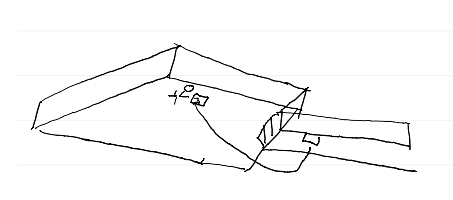
\includegraphics[width=1\linewidth]{content/pictures/Startroom_Sketch.png}
\caption{Sketchzeichnung des Hinweises für das erste Hindernis (Quelle: eigene Darstellung)}
\label{fig:sketch-startriddle}
\end{figure}

Abbildung \ref{fig:sketch-startriddle} zeigt eine erste Überlegung, dass eine Notiz im Startraum darauf aufmerksam macht, dass ein schwerer Gegenstand auf eine Druckplatte gestellt werden muss, durch welche die Tür zum anliegenden Flur öffnet.

Außerdem soll der erste Abschnitt das Tragen und Platzieren von Gegenständen enthalten. Es kann also ein Hindernis geben, das über eine Fackelhalterung oder ähnliches gelöst werden kann. Dadurch benötigt der Player einen Gegenstand, den er vom Watcher geschickt bekommt und an die entsprechende Stelle platzieren kann.

Das letzte Lernziel enthält das Freischalten von neuen Abschnitten, das sowohl für den Player als auch den Watcher gilt.

\paragraph{Beschreibung des Abschnittes}

\begin{figure}[ht]
\centering
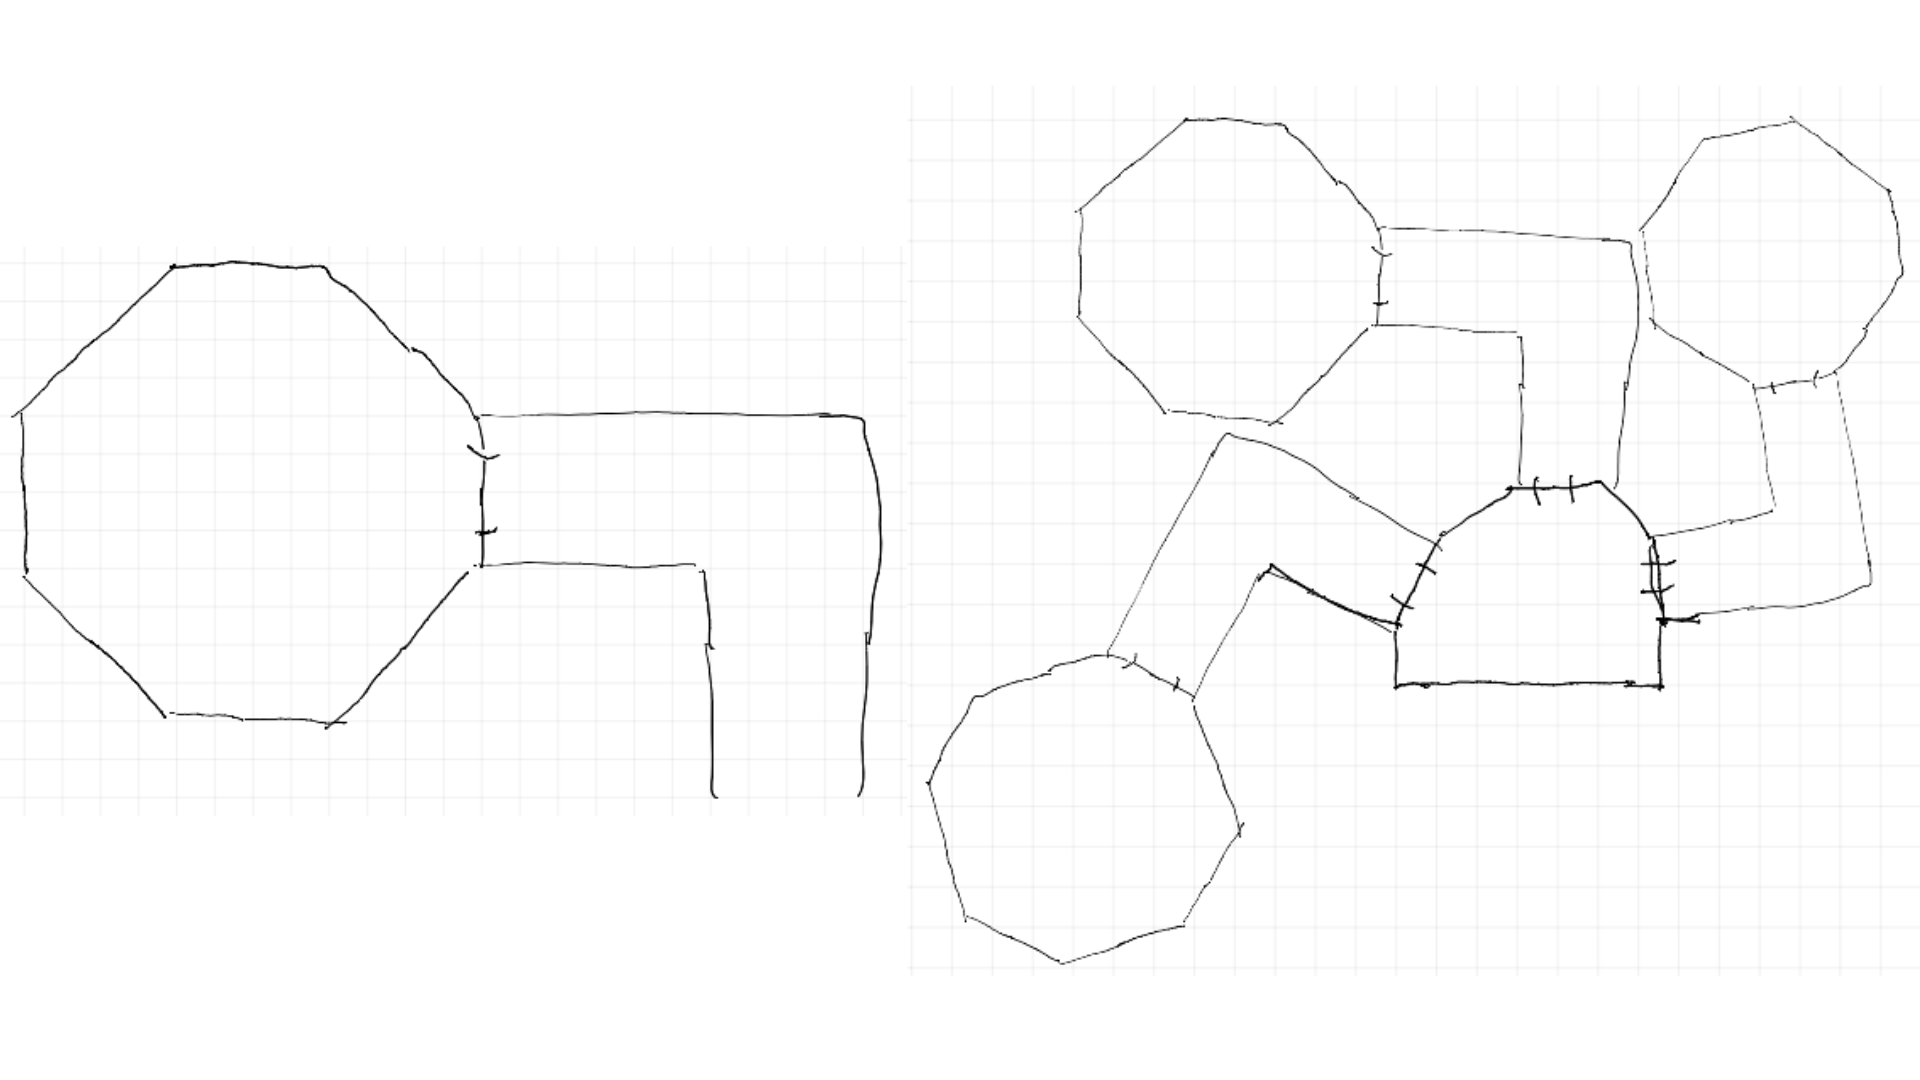
\includegraphics[width=1\linewidth]{content/pictures/Abschnitt_Concept_00.png}
\caption{Konzept Abschnitt 1 (Quelle: eigene Darstellung)}
\label{fig:section_00_concept}
\end{figure}

Abbildung \ref{fig:section_00_concept} zeigt eine erste Konzeptzeichnung des ersten Abschnittes. Sie beinhaltet links einen sechs-eckigen Raum, in dem der Spieler-Avatar des Players in die Spielwelt gesetzt wird. Diesen ersten Startraum gibt es, wie man auf der rechten Seite des Bildes sehen kann drei mal. Der Player muss seinem Watcher nun beschreiben in welchem der drei Räume er sich befindet. Die Räume unterscheiden sich dabei in ihrer Gestaltung. Wie in Abbildung \ref{fig:corridors} zu sehen, besitzt der erste Raum (erste Reihe, linkes Bild) einen Kronleuchter in der Mitte des Raumes, der zweite Raum (zweite Reihe, linkes Bild) einen großen Teppich und der dritte Raum (dritte Reihe, linkes Bild) eine Bank zwischen zwei Innensäulen.

\begin{figure}[ht]
\centering
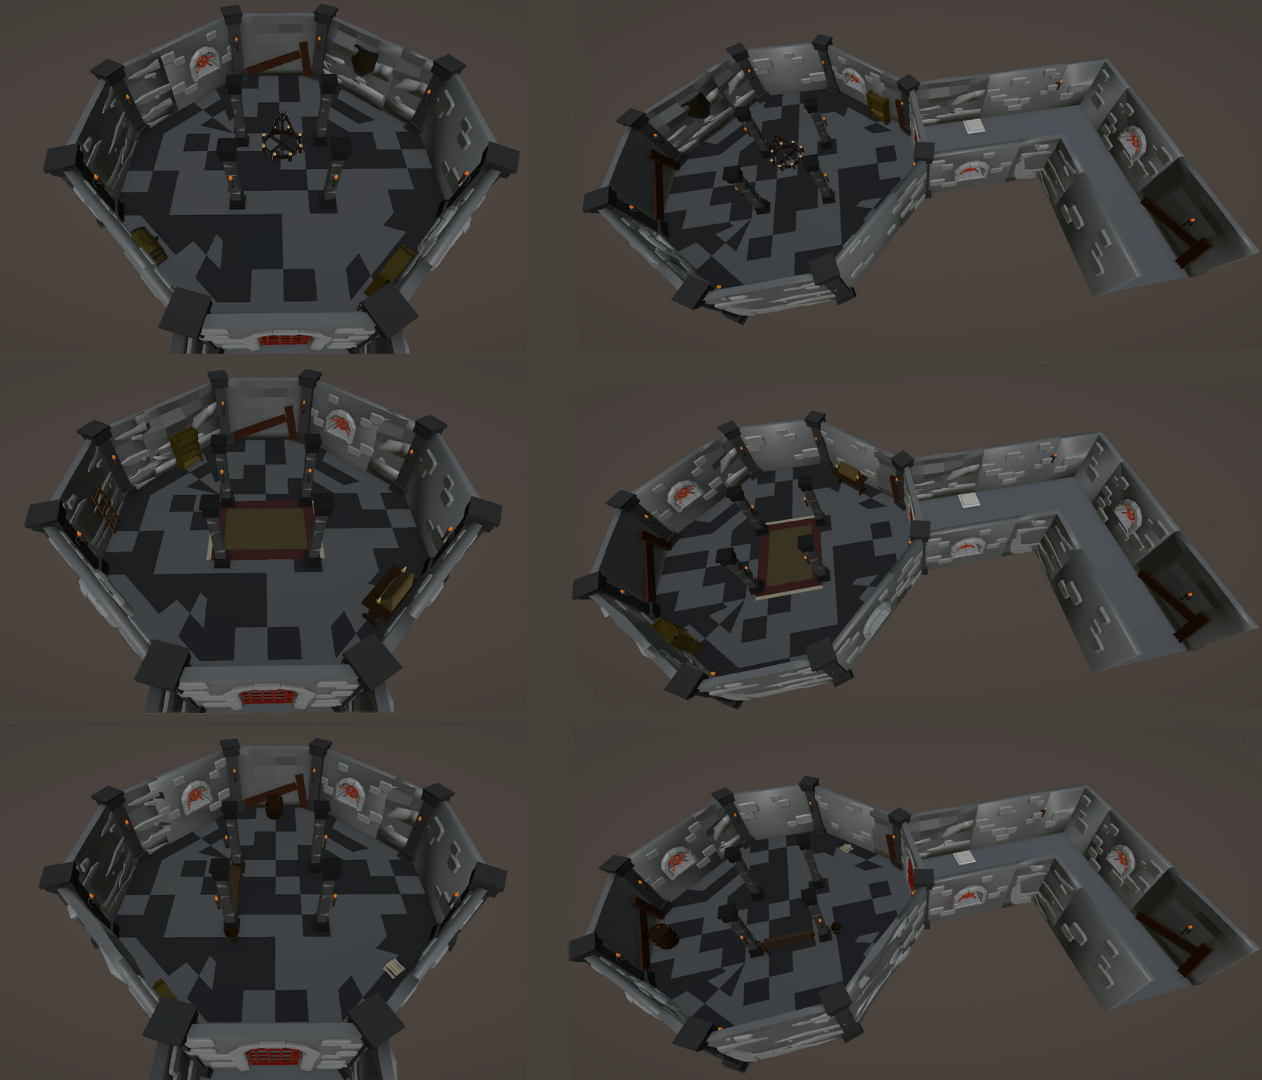
\includegraphics[width=1\linewidth]{content/pictures/Room_00-Room_02-Corridor_00-Corridor_02.png}
\caption{Korridor 1 bis Korridor 3 (Quelle: eigene Darstellung)}
\label{fig:corridors}
\end{figure}

Wie in der Konzeptzeichnung von Abbildung \ref{fig:section_00_concept} im rechten Bild zu sehen führen die Starträume über einen eckigen Flur in eine Eingangshalle. Dieser ist in Abbildung \ref{fig:section_00} zu sehen. An der entgegenfliegenden Wand von den drei eckigen Fluren aus ist eine Tür, durch die der Player mit Hilfe des Watchers gelangen muss um den folgenden Abschnitt freizuschalten. 

\begin{figure}[ht]
\centering
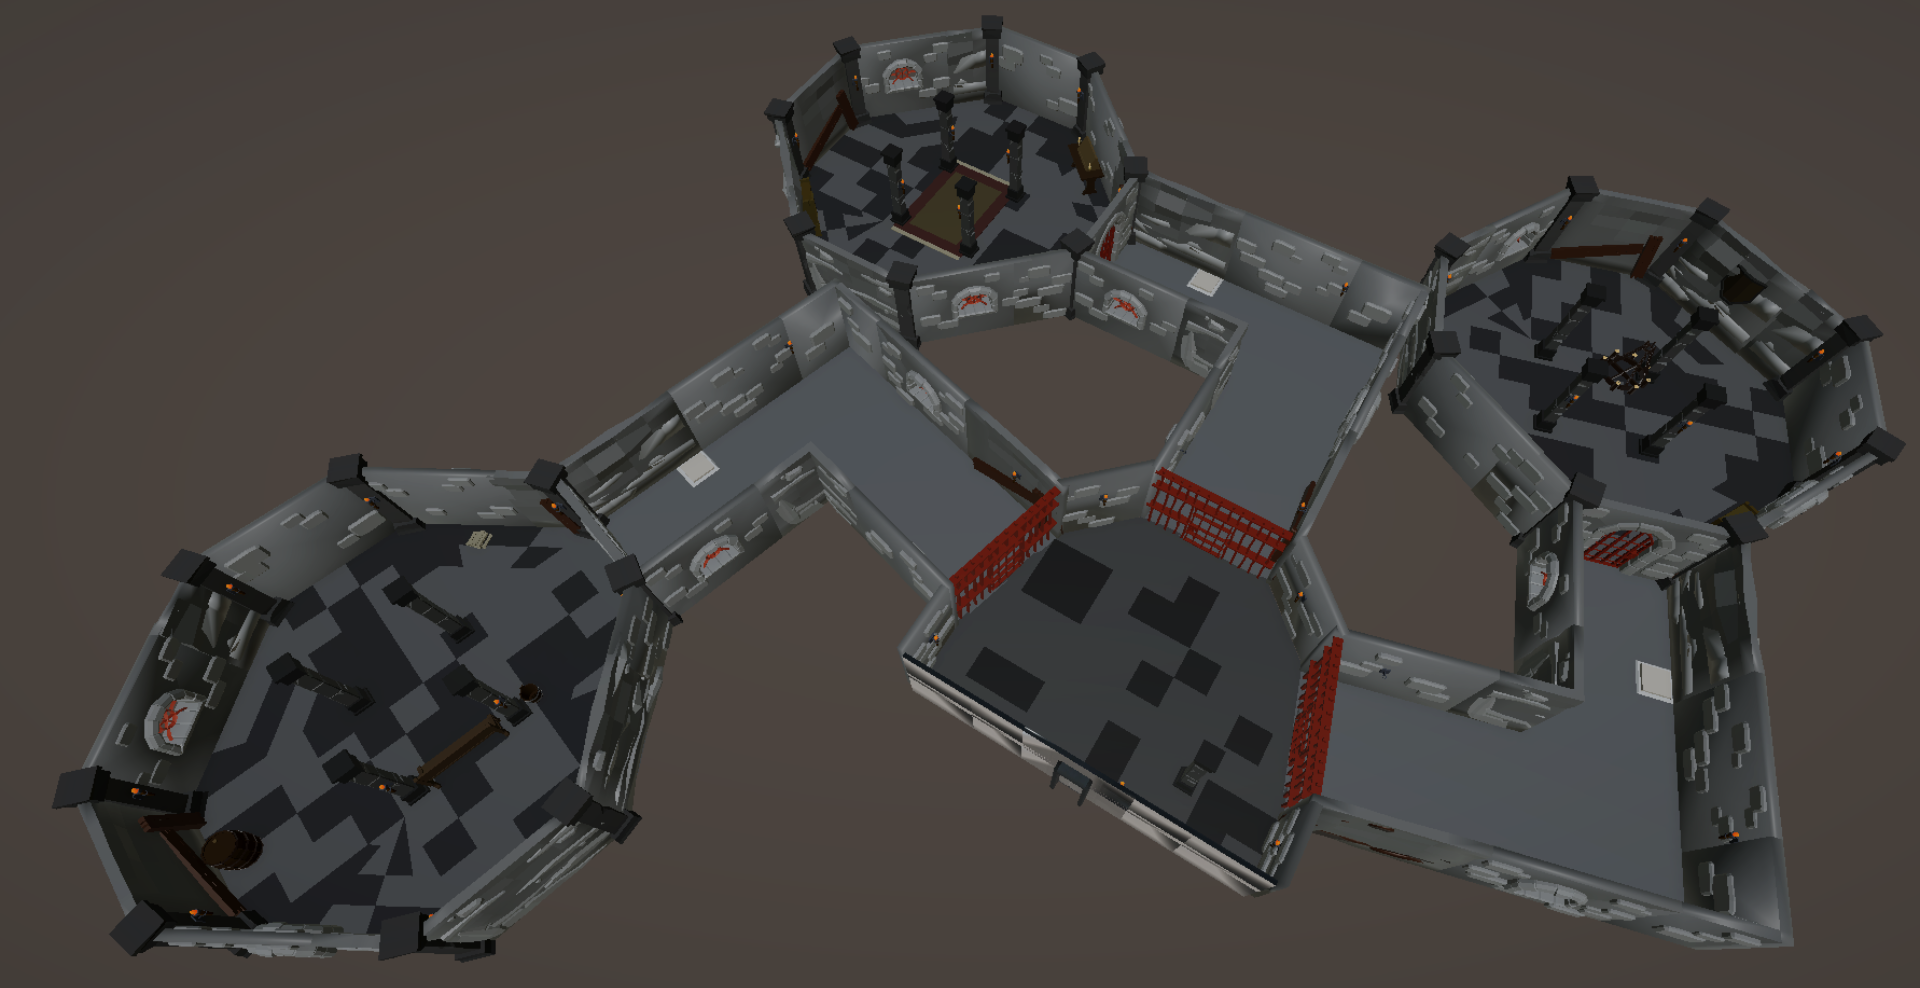
\includegraphics[width=1\linewidth]{content/pictures/Abschnitt_00.PNG}
\caption{Abschnitt 1 (Quelle: eigene Darstellung)}
\label{fig:section_00}
\end{figure}

Der Watcher sieht zum Start den gesamten ersten Abschnitt aus Abbildung \ref{fig:section_00}, wohingegen der Player nur einen der drei Starträume aus Abbildung \ref{fig:corridors} und den anliegenden Flur sehen kann. Die anderen zwei Räume samt Flur kann er nicht sehen. Auch dann nicht, wenn er in der Eingangskammer zum nächsten Abschnitt gelangt ist.

% \paragraph{Lernaspekte dieses Abschnittes}

\subsection{Abschnitt 2: Der Sicherheitsraum}
Analog zu Abschnitt 1 werden zunächst die Lernziele und konzeptionelle Überlegungen vorgestellt. Abschließend wird der Abschnitt vorgestellt.

\paragraph{Lernaspekte und Konzeption dieses Abschnittes}
Im zweiten Abschnitt erlernt der Watcher, dass er weitere Räume sehen kann, die der Player für ihn freigeschaltet hat. Der Player könnte in einem solchen Szenario einen Mechanismus in Gang gesetzt haben, durch welchen ein weiterer Raum für den Watcher sichtbar wurde und in ihm das Rätsel lösen muss.

Außerdem sieht er Gegenstände, welche der Player entdeckt hat als neue platzierte Gegenstände in der Welt und kann diese auch entfernen. Solch ein Gegenstand kann bspw. genutzt werden um ein weiteres Rätsel zu lösen.
In Abhängigkeit davon, erlernt der Player das Entdecken von Gegenständen, durch das nahe vorbei gehen an ihnen. Es kann so umgesetzt werden, dass der Player das Tooltip des Gegenstandes sieht und in diesem Moment der Gegenstand auch für den Watcher sichtbar wird.

\paragraph{Beschreibung des Abschnittes}

\begin{figure}[ht]
\centering
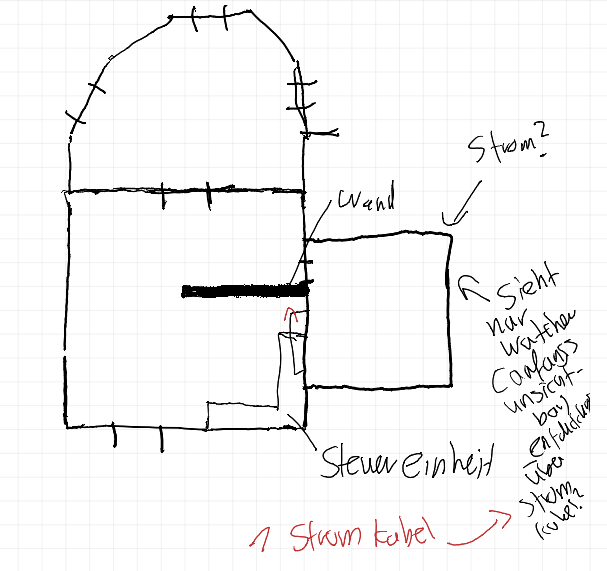
\includegraphics[width=1\linewidth]{content/pictures/Abschnitt_Concept_01.PNG}
\caption{Konzept Abschnitt 2 (Quelle: eigene Darstellung)}
\label{fig:section_01_concept}
\end{figure}

Abbildung \ref{fig:section_01_concept} zeigt eine erste Konzeptzeichnung des zweiten Abschnitts. Gedacht ist dieser als ein Sicherheitsraum, der ein Verbindungsstück zwischen dem zuvor beschriebenen Verlies ist und den folgenden Räumlichkeiten in Abschnitt 3. Der Player gelangt durch den oberen Eingang von der Eingangshalle in den Sicherheitsraum. Der Sicherheitsraum hat auf der rechten Seite eine Tür in einen Innenhof/ zu einem Außenbereich und kann durch die untere Tür in einen weiteren Abschnitt gelangen. Wichtig für einen Sicherheitsraum ist das Überwachungsterminal, welches in der unteren rechten Ecke des Raumes zu finden ist. Damit Arbeiter im Sicherheitsraum abgeschirmt von etwaigen anderen Mitarbeitern oder Personal ist, ist zwischen der Tür auf der rechten Seite und dem Terminal eine Trennwand eingebaut worden.

\begin{figure}[ht]
\centering
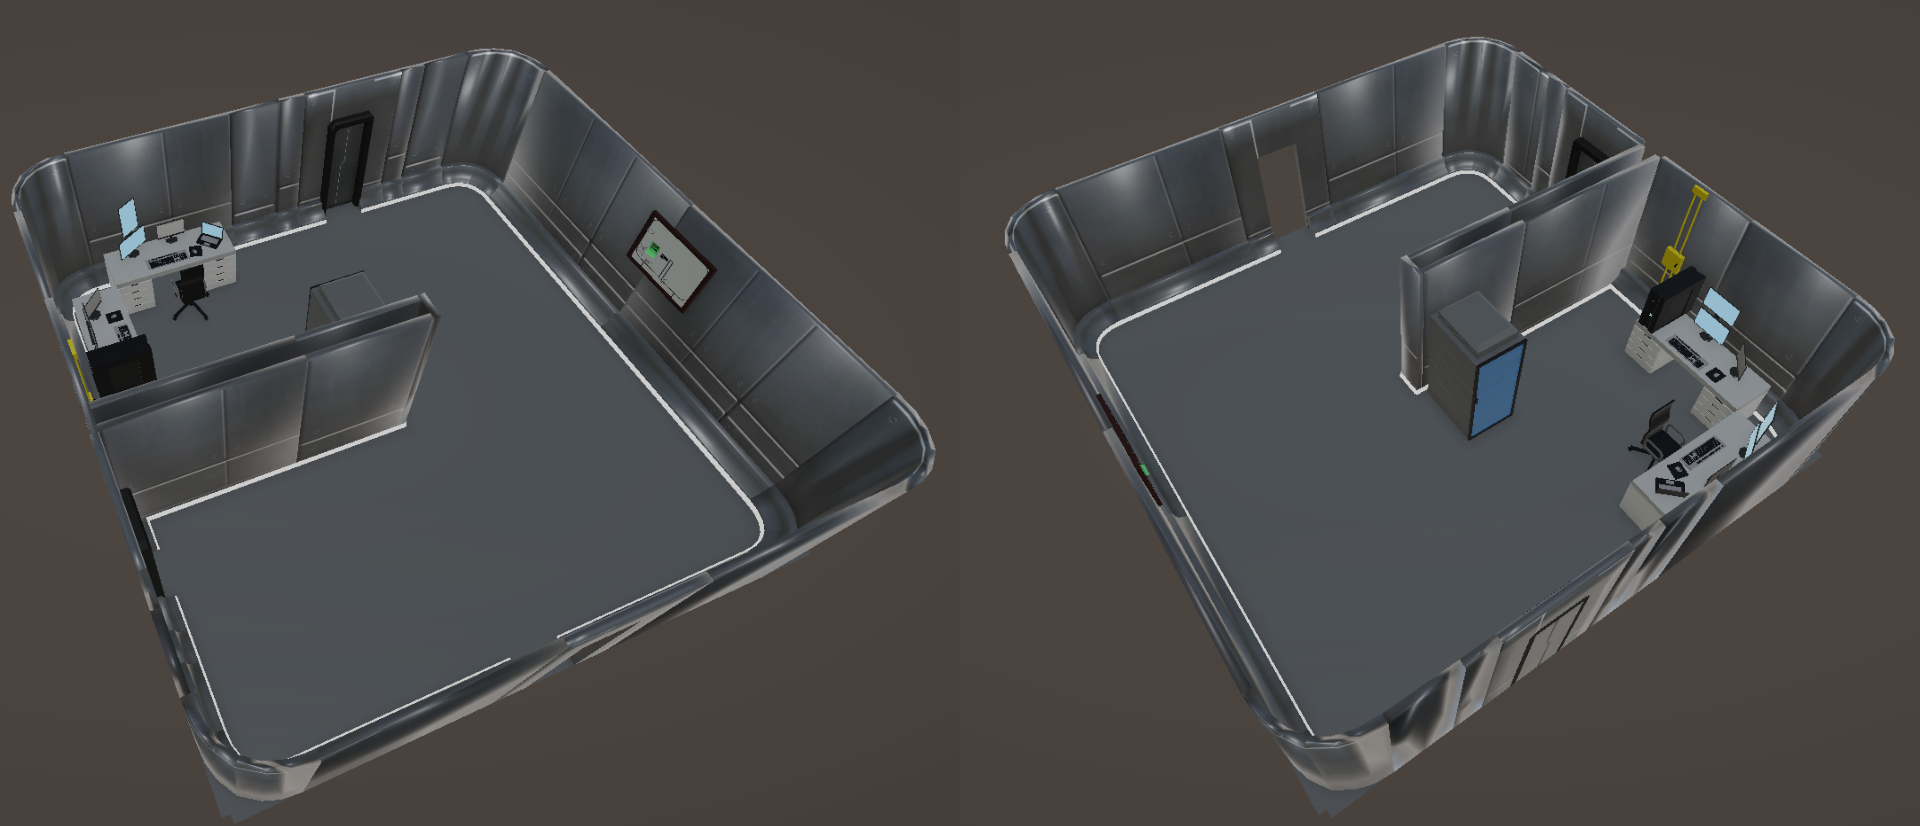
\includegraphics[width=1\linewidth]{content/pictures/Abschnitt_01 - Player.png}
\caption{Abschnitt 2 aus Sicht des Players (Quelle: eigene Darstellung)}
\label{fig:section_01_player}
\end{figure}

\begin{figure}[ht]
\centering
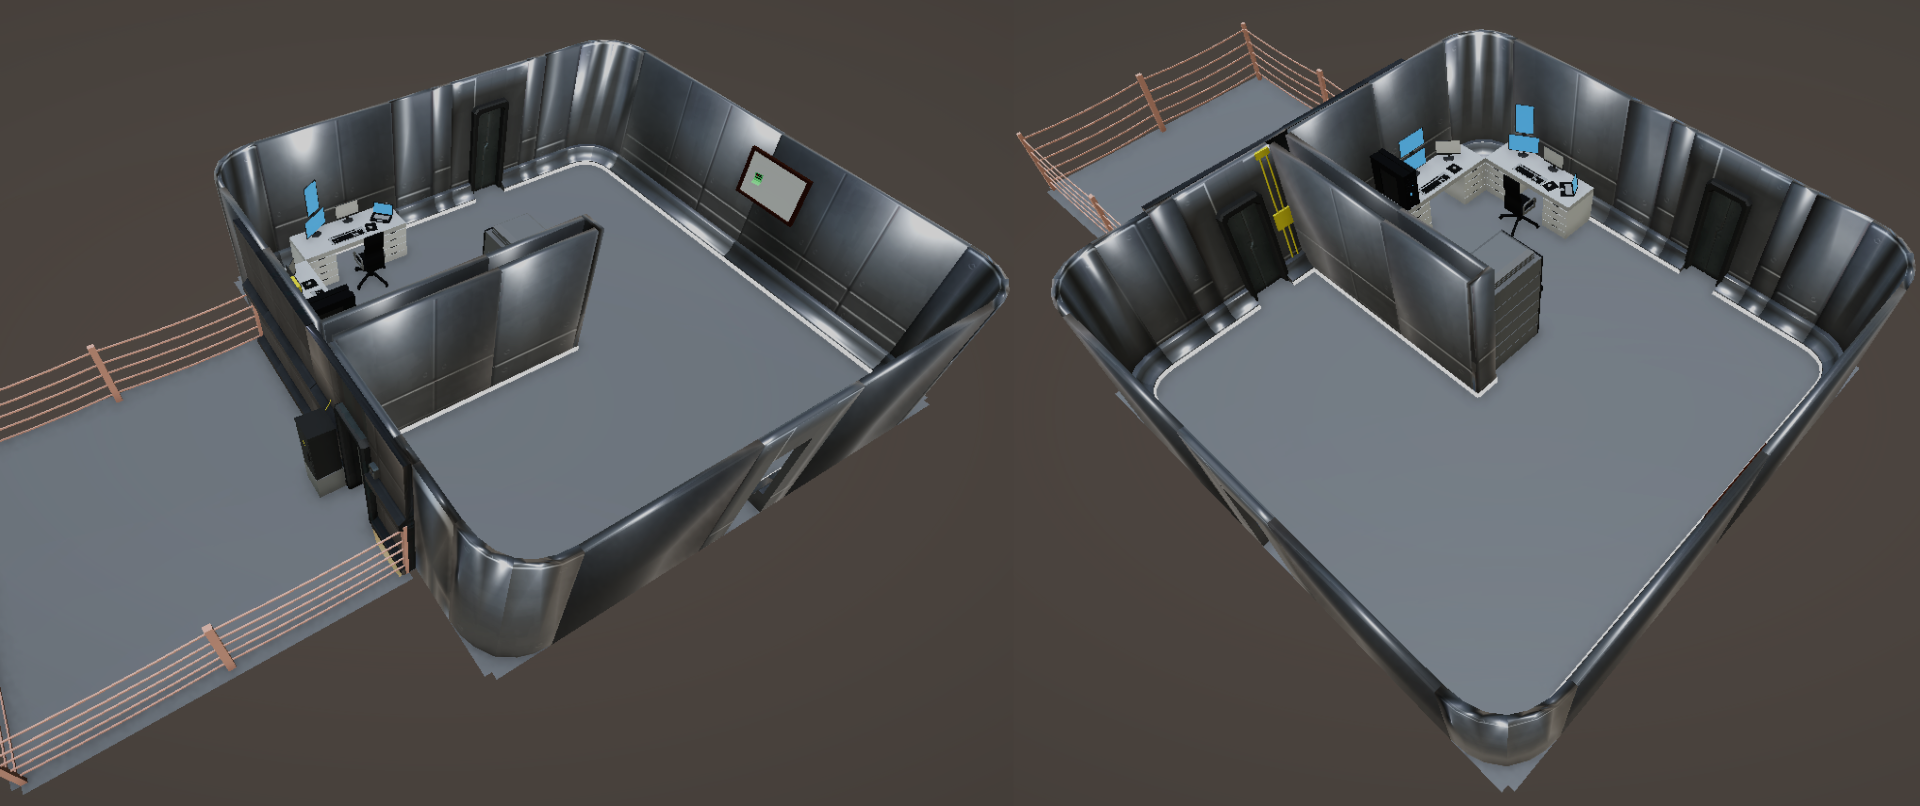
\includegraphics[width=1\linewidth]{content/pictures/Abschnitt_01 - Watcher.png}
\caption{Abschnitt 2 aus Sicht des Watchers (Quelle: eigene Darstellung)}
\label{fig:section_01_watcher}
\end{figure}

Die Abbildungen \ref{fig:section_01_player} und \ref{fig:section_01_watcher} zeigen den Sicherheitsraum in den Varianten der Ansicht von Player und Watcher. Die Unterschiede in den jeweiligen Szenen wurden gezielt so gewählt, dass sich Player und Watcher genauer absprechen müssen wie der Raum bei ihnen aufgebaut ist. Jeder Raum besitzt einen gelben Sicherungskasten mit gelben Leitungen die zu diesem Sicherungskasten hin- und wegführen. In Abbildung \ref{fig:section_01_player} steht dieser im rechten Bild links neben dem PC an der Rückwand zum Außenbereich. In der Anwendung des Watchers steht er im rechten Bild rechts neben der Tür zum Außenbereich (vgl. Abbildung \ref{fig:section_01_watcher}). Auf der Rückseite des Sicherungskasten befindet sich ein Stromgenerator, der im rechten Bild von Abbildung \ref{fig:section_01_watcher} links neben der Tür im Außenbereich zu sehen ist. Simultan zu dem Stromkasten der Player Anwendung fehlt dieser Stromkasten. Das ist für das enthaltene Rätsel wichtig. Wie in den beiden Abbildungen zu sehen ist, sieht nur die Anwendung des Watchers diesen Außenbereich mit dem Stromgenerator. Hier muss der Watcher selbständig durch die Hilfe des Players das enthaltene Rätsel lösen.

\subsection{Abschnitt 3: Das Büro}
Der dritte Abschnitt dient im Tutorial nicht mehr als Lernabschnitt sondern soll direkt als Anwendungsgebiet der erlernten Mechaniken dienen.
Als Szenario wurde hierbei ein Büroabschnitt innerhalb eines größeren Bürokomplexes gewählt. Dieser ist ein Teil des Bürokomplexes aus der Haupthandlung des Spiels. Der vorangegangene Abschnitt diente als Kontrollraum zwischen dem Verlies und dem Bürokomplex.

\begin{figure}[ht]
\centering
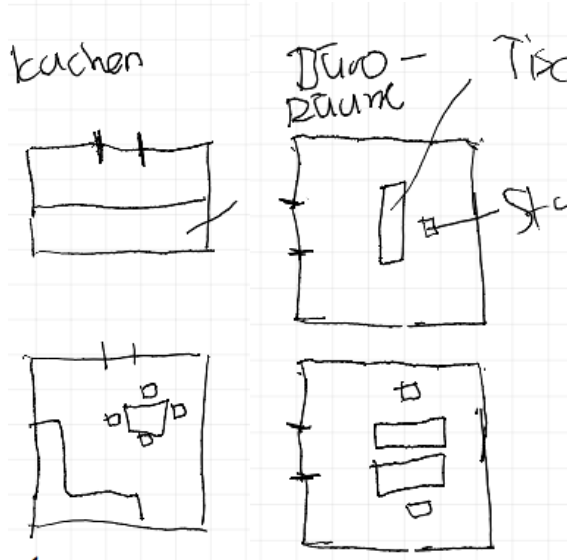
\includegraphics[width=1\linewidth]{content/pictures/Abschnitt_02_Concept.png}
\caption{Konzept Abschnitt 3 (Quelle: eigene Darstellung)}
\label{fig:section_02_concept}
\end{figure}

Abbildung \ref{fig:section_02_concept} zeigt erste Überlegungen für Räume innerhalb des Bürokomplexes. Diese ersten Überlegungen wurden in Abbildung \ref{fig:section_02} erweitert.

\begin{figure}[ht]
\centering
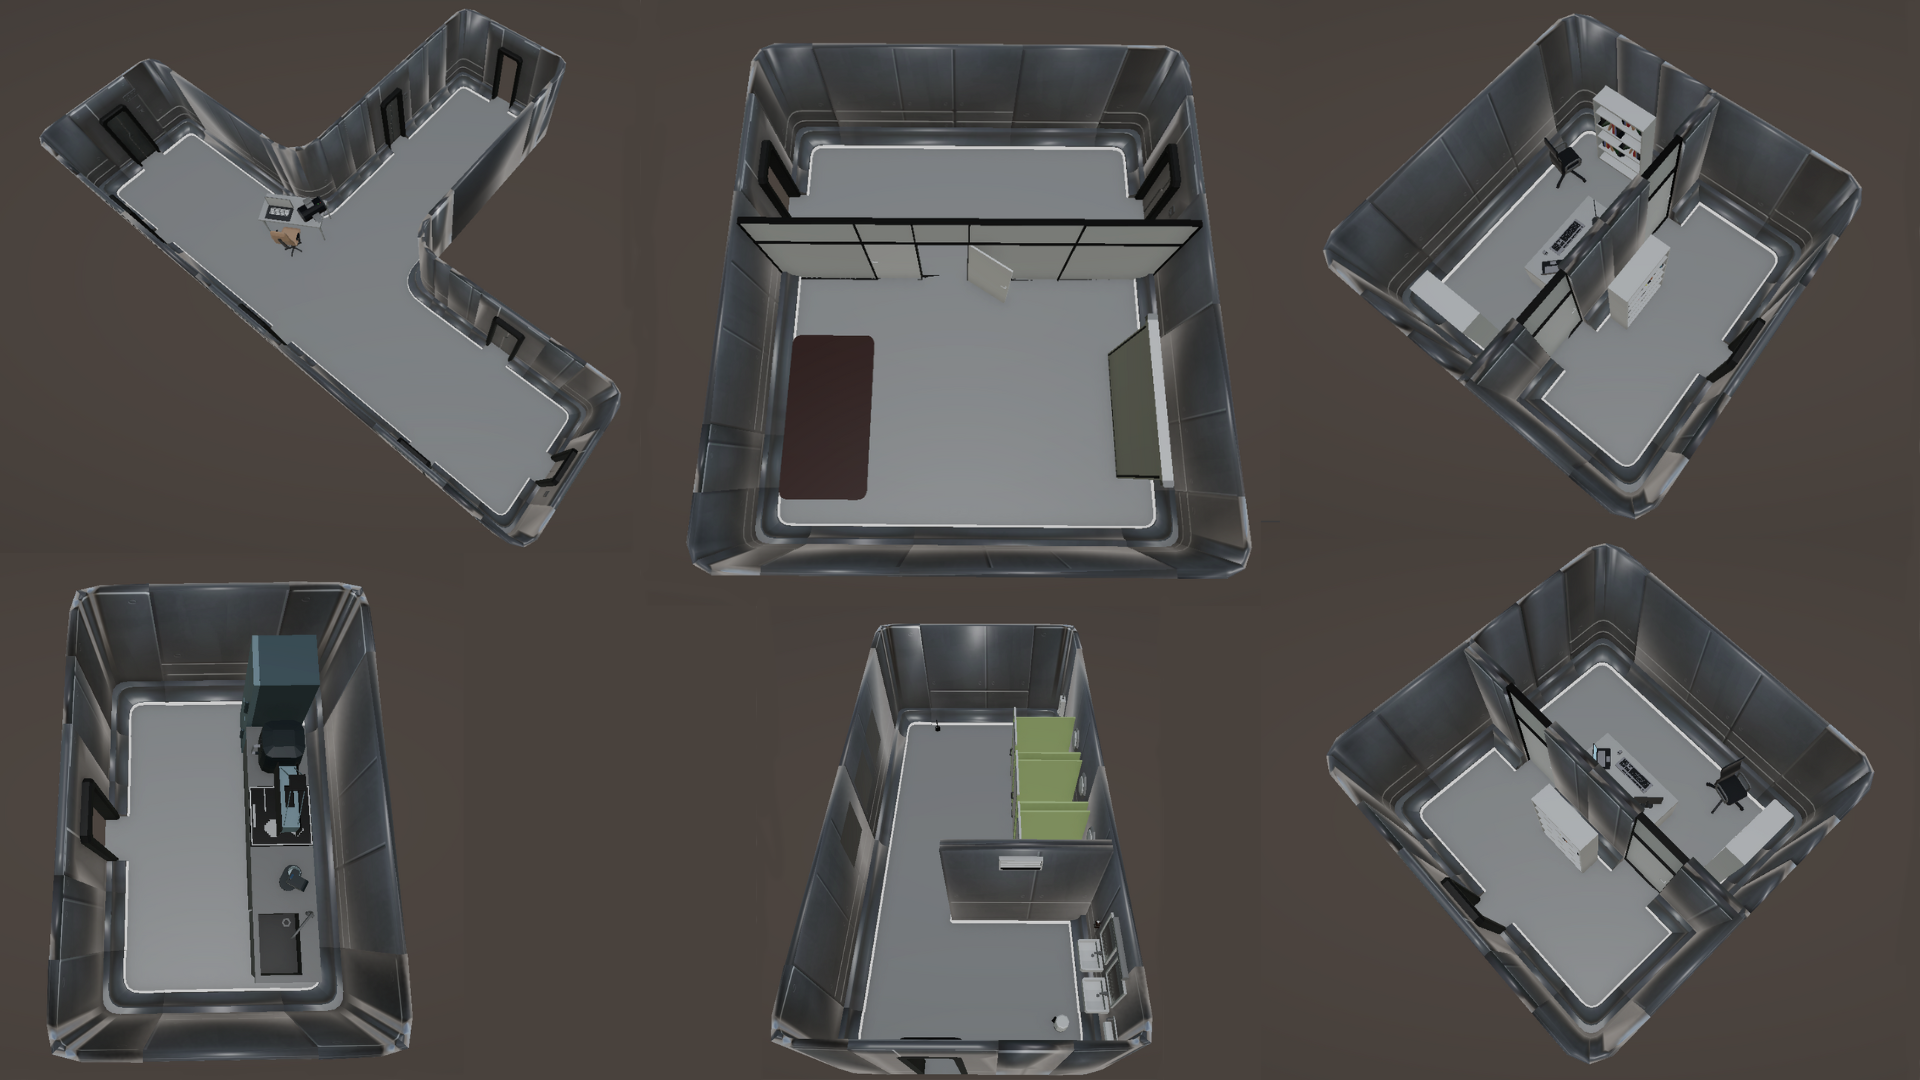
\includegraphics[width=1\linewidth]{content/pictures/Abschnitt_02.png}
\caption{Abschnitt 3 (Quelle: eigene Darstellung)}
\label{fig:section_02}
\end{figure}

Der Bürokomplex im letzten Teil des Tutorials besteht aus einem Korridor (Bild oben links), einer Küche (unten links), einem Tagungsraum (oben Mitte), einem kleinen WC (unten Mitte) und zwei Büros (oben und unten rechts). Auch hier existieren Unterschiede zwischen den Anwendungen des Players und des Watchers. Sowohl der Player als auch der Watcher sehen nur eines der beiden Büros. Sie sind zueinander gespiegelt und enthalten auch ein Rätsel und Hinweise darauf, wie nach Abschließen des enthaltenen Rätsel weiterzumachen ist. In der Anwendung des Players befinden sich im Tagungsraum Stühle, die vom Player entdeckt werden müssen, damit diese für den Watcher von Nutzen sein können. Wie die jeweiligen Räume zusammengehören und welchen Beitrag sie leisten wird im folgenden Kapitel \emph{\nameref{sec:riddles}} erklärt.

\subsection{Rätseldesign}\label{sec:riddles}
Der Aufbau der Rätsel in den Abschnitten 1 und 2 ist linear gehalten, da diese als Einführung in die Mechanik gedacht ist. Die Hinweise der Rätsel sind meist in der Nähe der jeweiligen Rätsel in die Umgebung, oder als Notiz, eingebaut.

\paragraph{Abschnitt 1}

\begin{figure}[ht]
\centering
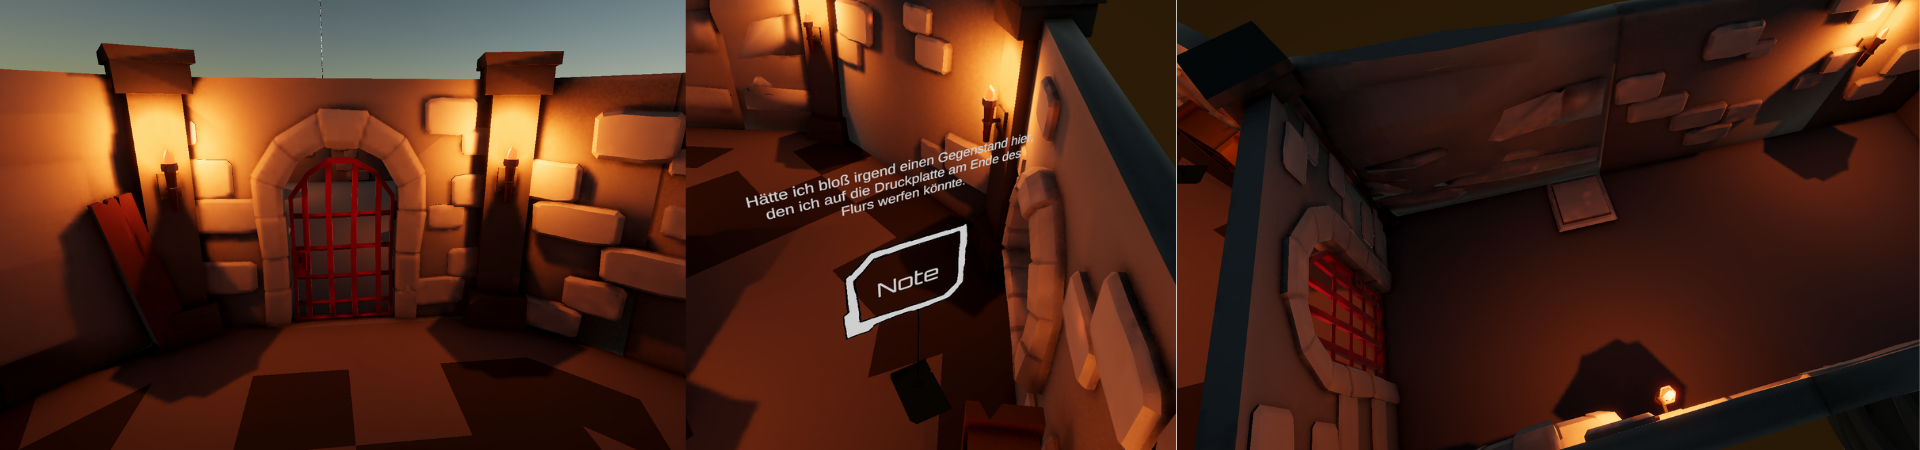
\includegraphics[width=1\linewidth]{content/pictures/Rätseldesign - Abschnitt00 - Rätsel00.png}
\caption{Aufbau der Rätsel von Abschnitt 1, Teil 1 (Quelle: eigene Darstellung)}
\label{fig:riddle-design-section00-00}
\end{figure}

\begin{figure}[ht]
\centering
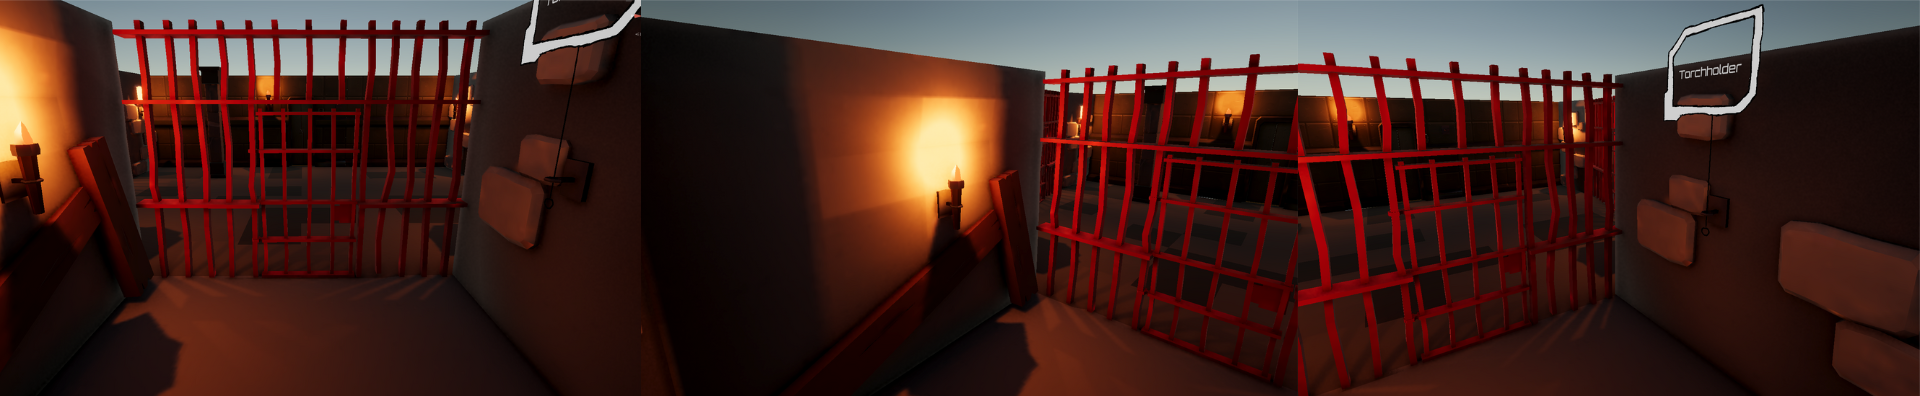
\includegraphics[width=1\linewidth]{content/pictures/Rätseldesign - Abschnitt00 - Rätsel01.png}
\caption{Aufbau der Rätsel von Abschnitt 1, Teil 2 (Quelle: eigene Darstellung)}
\label{fig:riddle-design-section00-01}
\end{figure}

\begin{figure}[ht]
\centering
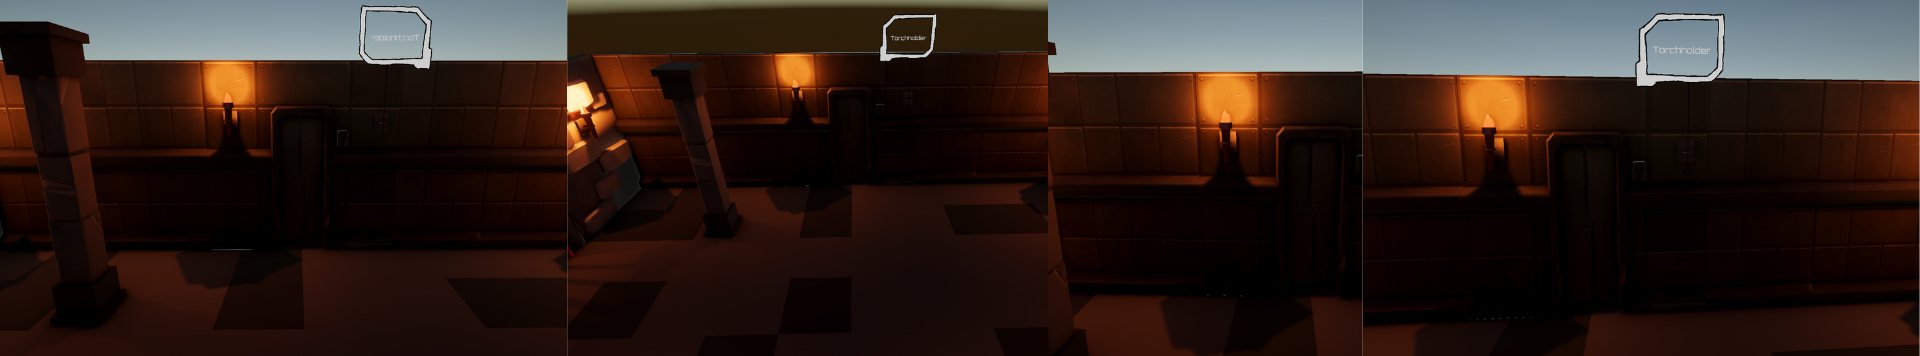
\includegraphics[width=1\linewidth]{content/pictures/Rätseldesign - Abschnitt00 - Rätsel02.png}
\caption{Aufbau der Rätsel von Abschnitt 1, Teil 3 (Quelle: eigene Darstellung)}
\label{fig:riddle-design-section00-02}
\end{figure}

Zum Start befindet sich der Player innerhalb des Verlieses. Eine verrostete Eisentür versperrt ihm den Weg aus dem Verlies (vgl. Abbildung \ref{fig:riddle-design-section00-00}, linkes Bild). Auf einer Notiz (vgl. Abbildung \ref{fig:riddle-design-section00-00}, mittleres Bild) erhält der Player einen Hinweis darauf, auf einer Druckplatte (vgl. Abbildung \ref{fig:riddle-design-section00-00}, rechtes Bild) etwas zu werfen. In diesem Fall ist damit das Platzieren eines schweren Gegenstandes (eine Säule) gemeint, welches zum Start des Spiels im Inventar des Watchers zu finden ist. 

Nachdem der Player aus dem Verlies gelangt ist, stößt er erneut auf eine verrostete Eisentür, welche ebenfalls geöffnet werden muss (vgl. Abbildung \ref{fig:riddle-design-section00-01}, linkes Bild). Auf der von der Tür aus linken Wand, sehen sowohl der Player als auch der Watcher eine Fackelhalterung, in der eine Fackel hängt (vgl. Abbildung \ref{fig:riddle-design-section00-01}, mittlere Bild). Außerdem befindet sich auf der entgegen liegenden Wandseite eine Fackelhalterung ohne Fackel (vgl. Abbildung \ref{fig:riddle-design-section00-01}. rechts Bild). Sie schließen daraus, dass der Watcher dem Player eine Fackel schicken und dieser sie in die Halterung einsetzen muss.

In der folgenden Eingangshalle stoßen beide Spieler auf eine verschlossene Sicherheitstür, welche zum Abschließen des Abschnittes geöffnet werden muss (vgl. Abbildung \ref{fig:riddle-design-section00-02}, linkes Bild). In der Eingangshalle befinden sich links von der Tür eine Säule und eine Fackelhalterung in der eine Fackel steckt (vgl. Abbildung \ref{fig:riddle-design-section00-02}, zweites Bild von links und zweites Bild von rechts). Auf der rechten Seite befindet sich eine leere Fackelhalterung (vgl. Abbildung \ref{fig:riddle-design-section00-02}, rechts Bild). Der Player muss die Fackel, die im vorherigen Rätsel verwendet wurde in die leere Halterung einsetzen. Außerdem muss der Watcher, gemäß der Beschreibung der Säule \say{The column is required to match a pattern or to serve as a counterweight.}, die Säule aus dem ersten Rätsel ungefähr an die auf der rechten Seite der Tür entgegen liegenden Stelle platzieren, sodass die Säulen symmetrisch zur Tür ausgerichtet sind (vgl. Abbildung \ref{fig:riddle-design-section00-02}, linkes Bild).

\paragraph{Abschnitt 2}
In Abschnitt 2 erfolgt das Rätseldesign ähnlich linear wie in Abschnitt 1.

\begin{figure}[ht]
\centering
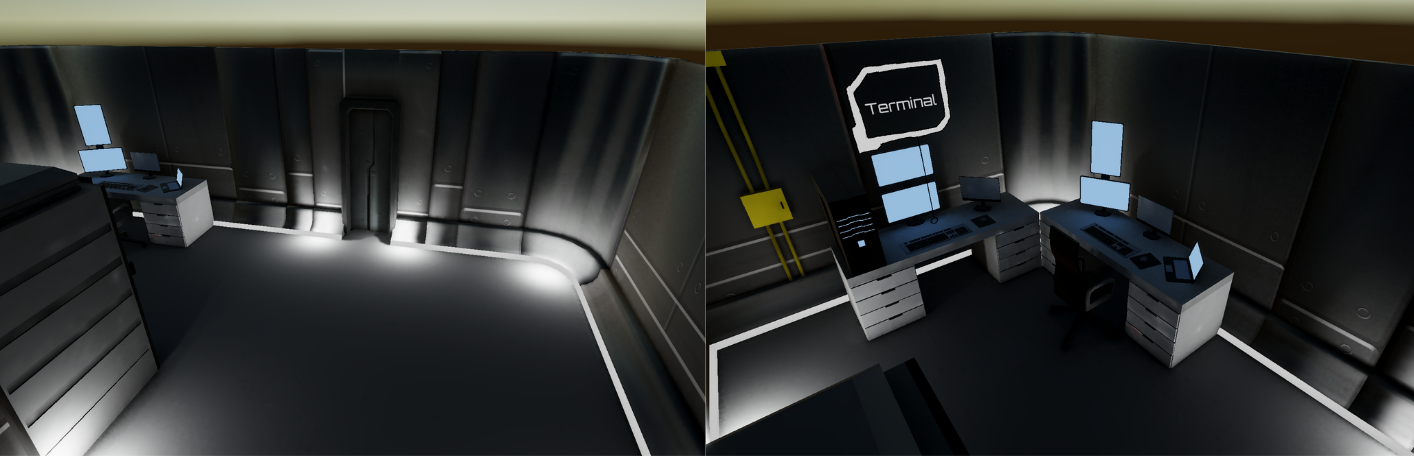
\includegraphics[width=1\linewidth]{content/pictures/Rätseldesign - Abschnitt01 - Rätsel00.png}
\caption{Aufbau der Rätsel von Abschnitt 2, Teil 1 (Quelle: eigene Darstellung)}
\label{fig:riddle-design-section01-00}
\end{figure}

\begin{figure}[ht]
\centering
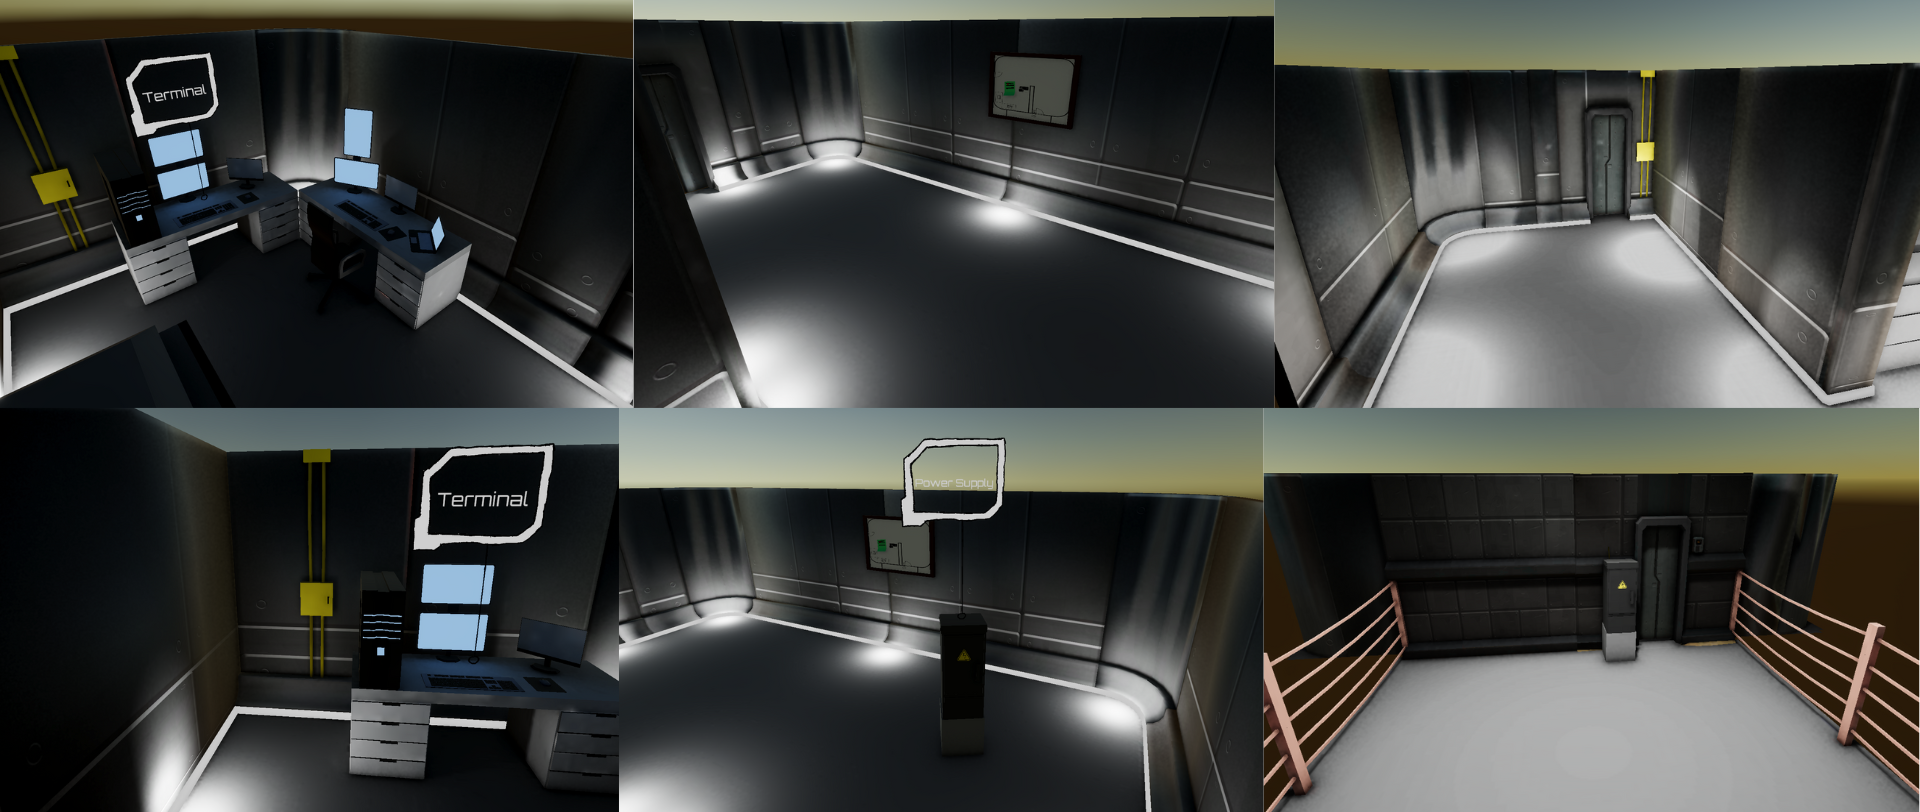
\includegraphics[width=1\linewidth]{content/pictures/Rätseldesign - Abschnitt01 - Rätsel01.png}
\caption{Aufbau der Rätsel von Abschnitt 2, Teil 2 (Quelle: eigene Darstellung)}
\label{fig:riddle-design-section01-01}
\end{figure}

Nachdem der Player in den Sicherheitsraum gegangen ist, stößt er auf 2 Türen. Eine links vom Eingang und die andere geradeaus durch. Durch die letztere muss der Player am Ende des Abschnittes gehen. Allerdings geht das zunächst nicht, da der Bewegungsmelder der Tür deaktiviert ist und erst aktiviert werden muss. Am Terminal, das links neben der Tür zu finden ist, muss er Player den Bewegungsmelder aktivieren (vgl. Abbildung \ref{fig:riddle-design-section01-00}). Allerdings besitzt dieses keinen Strom. 

Der Player als auch der Watcher erhalten einige Hinweise darauf, wie der Strom für das Terminal zu aktivieren ist. Zunächst befindet sich innerhalb des Sicherheitsraumes ein Stromgenerator (vgl. Abbildung \ref{fig:riddle-design-section01-01}, Bild zweite Zeile Mitte), welcher an einen anderen Ort platziert werden muss. In der Ansicht des Watchers befindet sich rechts neben der zweiten Tür im Sicherheitsraum, die vom Eingang in den Raum aus links ist, eine Sicherung, auf deren anderen Seite in einem kleinen Innenhof ein Stromgenerator für die Eingangstür steht (vgl. Abbildung \ref{fig:riddle-design-section01-01}, Bilder erste und zweite Zeile rechts). Der Player besitzt für diesen Aufbau, den der Watcher in seiner Version sieht, einen Plan auf einer Pinnwand (vgl. Abbildung \ref{fig:riddle-design-section01-01}, Bild erste Reihe Mitte). Der Unterschied zwischen der Version des Players und des Watchers ist, dass die Sicherung nicht neben der Tür ist, sondern links neben dem Terminal (vgl. Abbildung \ref{fig:riddle-design-section01-01}, Bild zweite reihe links). Aus diesem Grund muss der Generator auf die entgegenfliegende Seite links neben den bestehenden Stromkasten in der Anwendung des Watchers (vgl. Abbildung \ref{fig:riddle-design-section01-01}, Bild zweite Reihe rechts) platziert werden. Ist der Generator an die Stelle platziert, kann der Bewegungsmelder über das Terminal aktiviert werden und der Player kann Abschnitt 3 betreten.

\paragraph{Abschnitt 3}
Abschnitt 3 ist der komplexeste des Tutorials. Player und Watcher erhalten in verschiedenen freigeschalteten Räumen Hinweise oder Gegenstände zu weiteren Rätseln die bei Rätseln zu späteren Zeitpunkten benötigt werden.

\begin{figure}[ht]
\centering
\includegraphics[width=0.7\linewidth]{content/pictures/Rätseldesign_Section02.drawio.png}
\caption{Rätseldesign von Abschnitt 3 (Quelle: eigene Darstellung), vollständig in Anhang: \ref{}}
\label{fig:r
iddle-design-section02-uml}
\end{figure}

Abbildung \ref{fig:riddle-design-section02-uml} zeigt das für das in Abschnitt 3 entworfene Rätseldesign. Dieses Diagramm wird durch die Abbildungen \ref{fig:riddle-design-section02-00} bis \ref{fig:riddle-design-section02-04} vervollständigt.

\begin{figure}[ht]
\centering
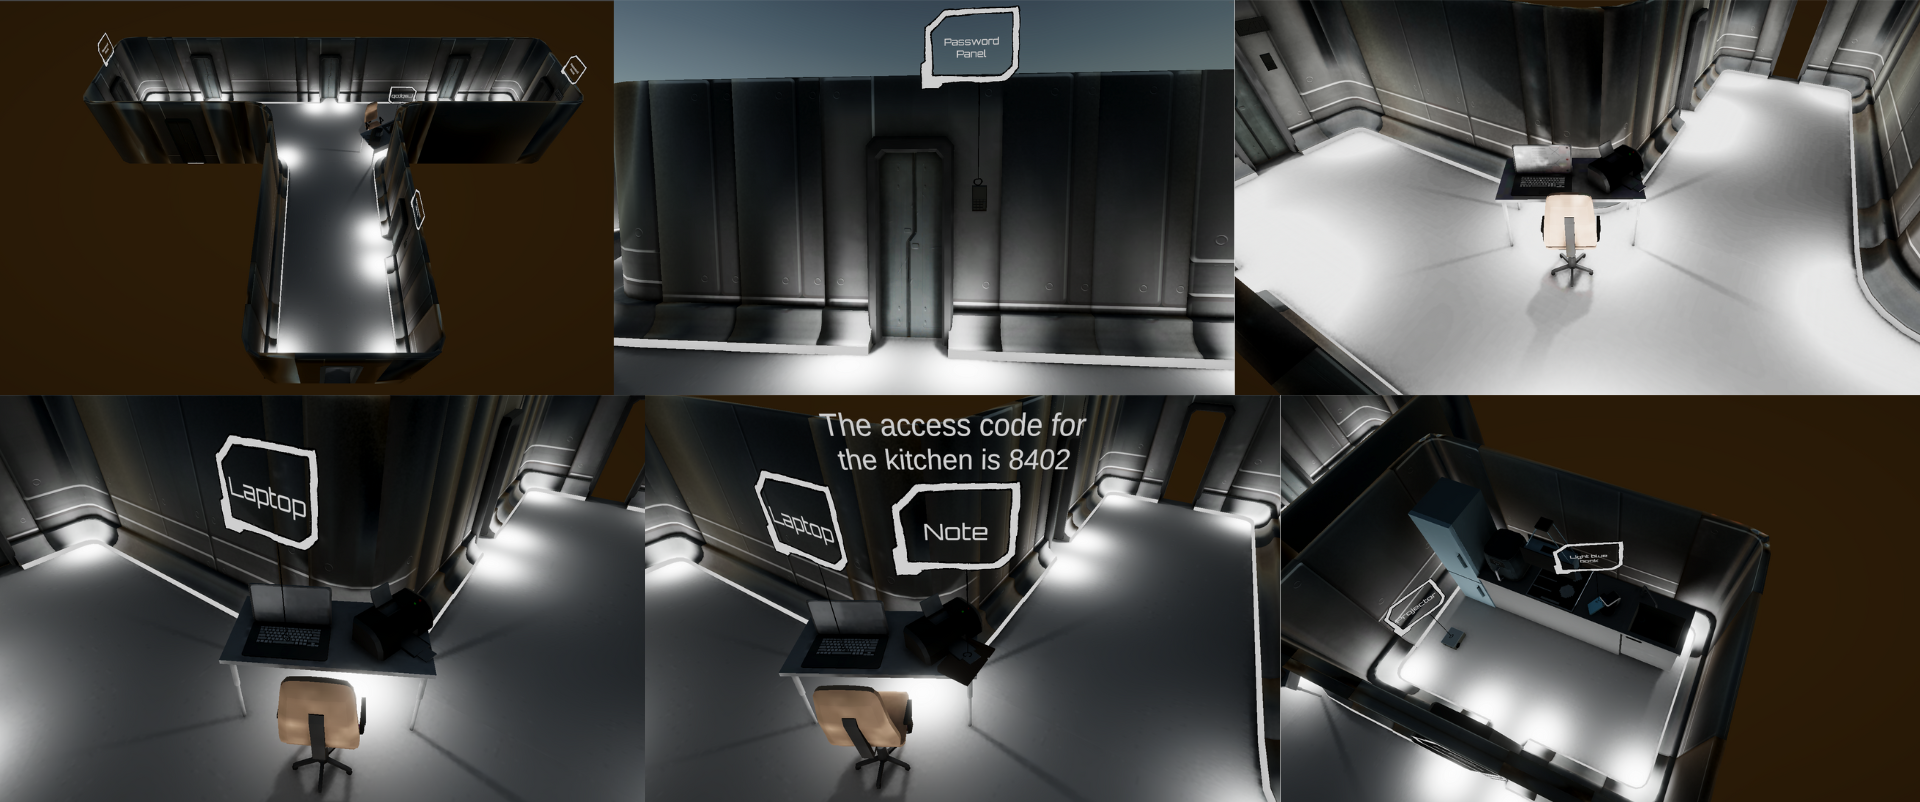
\includegraphics[width=1\linewidth]{content/pictures/Rätseldesign - Abschnitt02 - Rätsel00.png}
\caption{Aufbau der Rätsel von Abschnitt 3, Teil 1 (Quelle: eigene Darstellung)}
\label{fig:riddle-design-section02-00}
\end{figure}

\begin{figure}[ht]
\centering
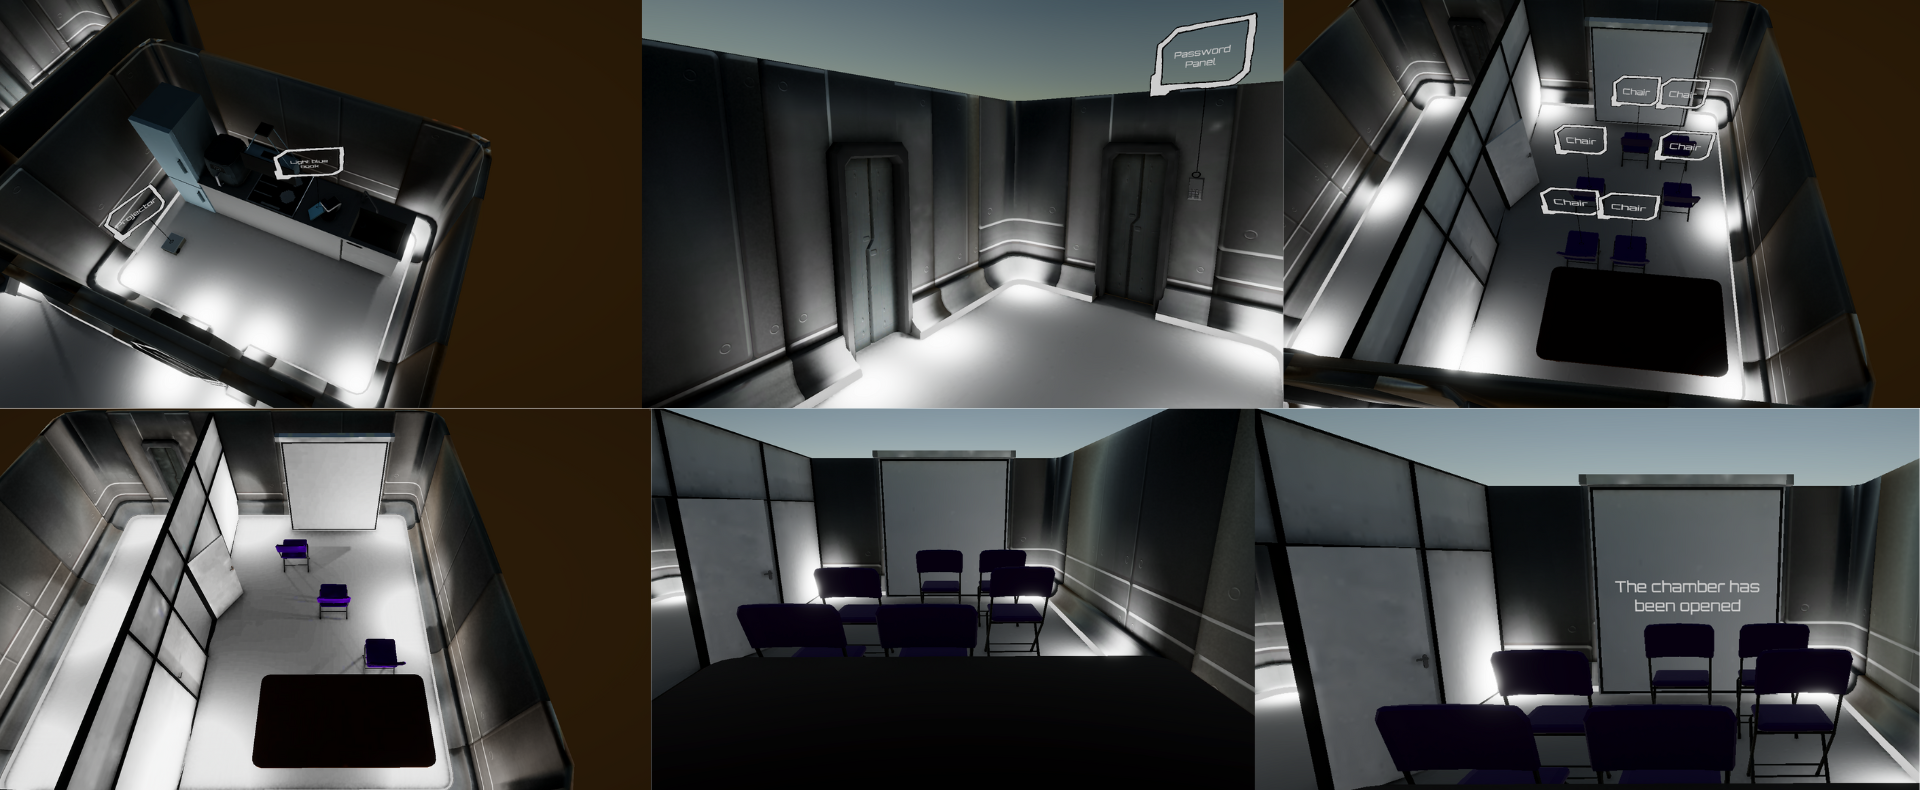
\includegraphics[width=1\linewidth]{content/pictures/Rätseldesign - Abschnitt02 - Rätsel01.png}
\caption{Aufbau der Rätsel von Abschnitt 3, Teil 2 (Quelle: eigene Darstellung)}
\label{fig:riddle-design-section02-0l}
\end{figure}

\begin{figure}[ht]
\centering
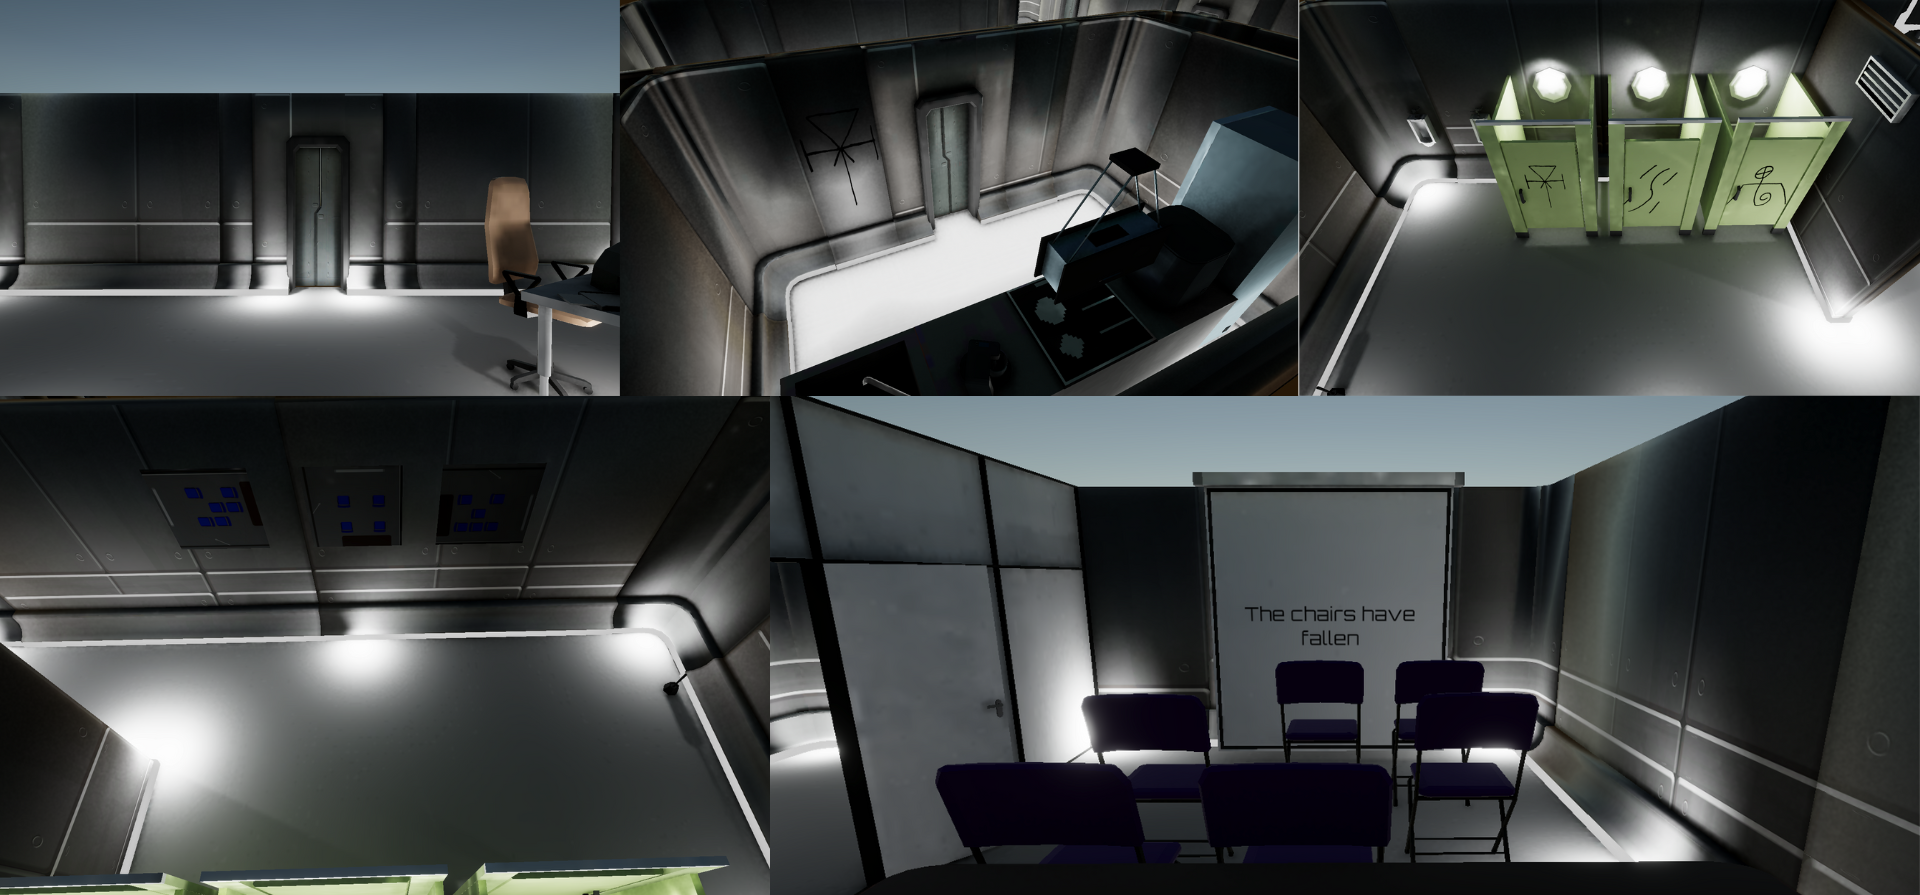
\includegraphics[width=1\linewidth]{content/pictures/Rätseldesign - Abschnitt02 - Rätsel02.png}
\caption{Aufbau der Rätsel von Abschnitt 3, Teil 3 (Quelle: eigene Darstellung)}
\label{fig:riddle-design-section02-02}
\end{figure}

\begin{figure}[ht]
\centering
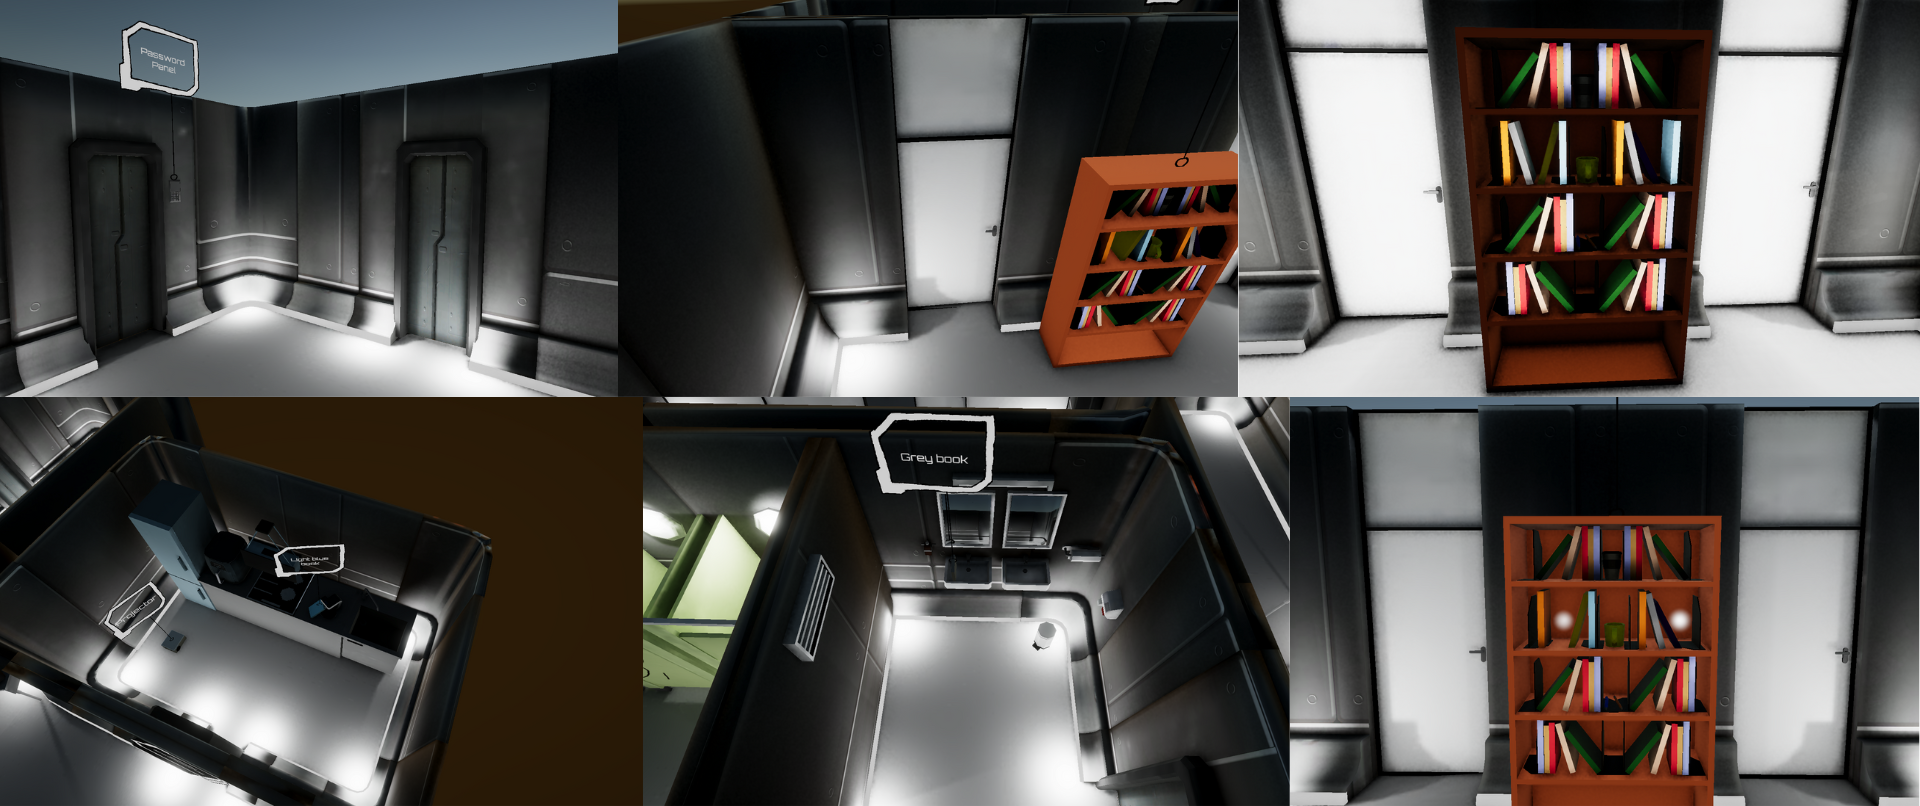
\includegraphics[width=1\linewidth]{content/pictures/Rätseldesign - Abschnitt02 - Rätsel03.png}
\caption{Aufbau der Rätsel von Abschnitt 3, Teil 4 (Quelle: eigene Darstellung)}
\label{fig:riddle-design-section02-03}
\end{figure}

\begin{figure}[ht]
\centering
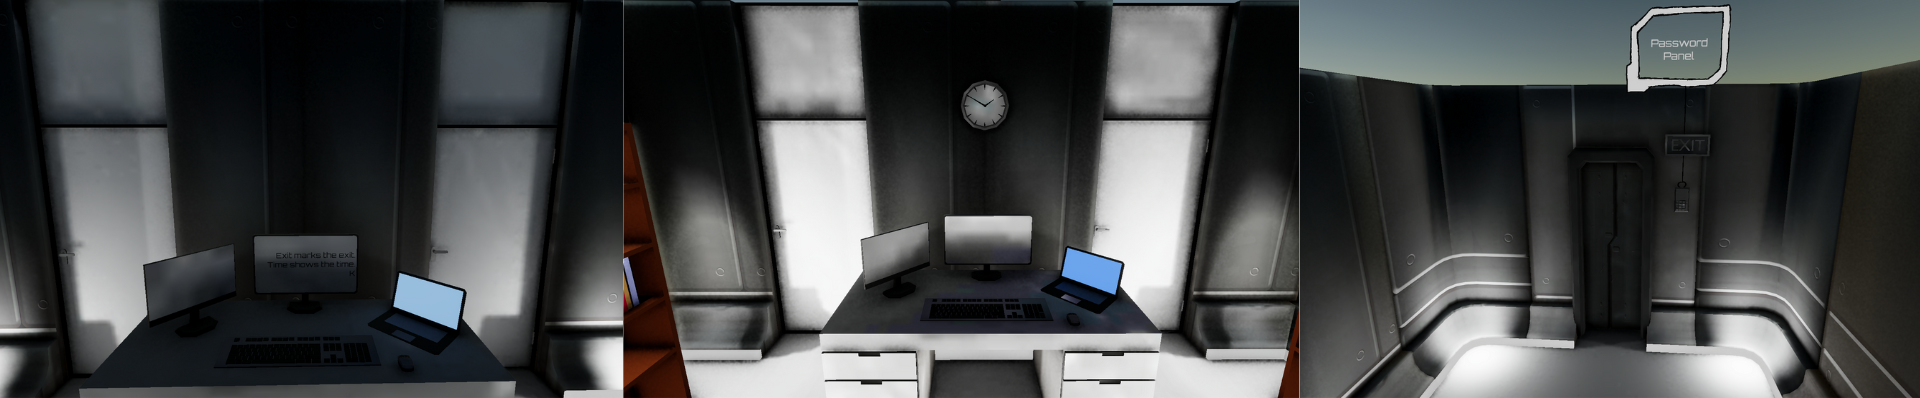
\includegraphics[width=1\linewidth]{content/pictures/Rätseldesign - Abschnitt02 - Rätsel04.png}
\caption{Aufbau der Rätsel von Abschnitt 3, Teil 5 (Quelle: eigene Darstellung)}
\label{fig:riddle-design-section02-04}
\end{figure}

Nachdem der Player den neuen Korridor betreten hat, stößt er auf einige verschlossene Türen (vgl. Abbildung \ref{fig:riddle-design-section02-00}, Bild erste Reihe links). Zum Start muss der Player den Druckbefehl starten, welcher in der Watcher Anwendung am Laptop zu sehen ist (vgl. Abbildung \ref{fig:riddle-design-section02-00}, Bild zweite Reihe links). Wurde der Druckvorgang gestartet, erhält der Player eine Notiz mit der Zahlenkombination zur Küche (vgl. Abbildung \ref{fig:riddle-design-section02-00}, Bild zweite Reihe Mitte). Der Watcher sieht zu diesem Zeitpunkt bereits die Küche und muss den Player zur Küche navigieren. In der Küche angekommen entdeckt der Player einen Projektor und ein Buch, welche zu späteren Rätseln gebraucht werden (vgl. Abbildung \ref{fig:riddle-design-section02-00}, Bild zweite Reihe rechts). 

Sobald der Projektor entdeckt und auch beim Watcher angezeigt wurde, öffnet sich das Konferenzzimmer (vgl. Abbildung \ref{fig:riddle-design-section02-0l}, Bild erste Reihe Mitte und Bild erste Reihe Rechts). Der Player als auch der Watcher sehen Stühle im Innenbereich des großen Konferenzraums. Anzumerken ist hier, dass sich die Anzahl der Stühle jeweils in den Anwendungen entscheiden. So erscheinen beim Watcher alle Stühle, zusätzlich zu den bereits existierenden, nachdem der Player diese entdeckt (vgl. Abbildung \ref{fig:riddle-design-section02-0l}, Bild erste Reihe rechts und zweite Reihe links). Nachdem der Watcher den gefundenen Projektor auf den Tisch platziert, erscheint eine Nachricht auf der Leinwand und das Team muss weiter ins Badezimmer (der Spruch \say{The chamber has been opened} orientiert sich dabei an den Spruch der Kammer des Schreckens aus Harry Potter 2 und bezieht sich dabei auf das anliegende WC) (vgl. Abbildung \ref{fig:riddle-design-section02-0l}, Bild zweite Reihe Mitte und zweite Reihe rechts).

Im Badezimmer erhält der Player einen Hinweis darauf, was der Watcher mit den Stühlen im Konferenzzimmer machen muss. An den Türen der Toilettenkabinen befinden sich drei verschiedene Symbole (Die Symbole wurden aus dem Spiel \say{We were here too} entnommen (vgl. \cite{noauthor_we_nodate})) die jeweils für die Anordnungen der Stühle stehen. Die Abbildungen der Anordnungen befinden sich auf den an der Wand hängenden Postern (vgl. Abbildung \ref{fig:riddle-design-section02-02}, Bild erste Reihe rechts und zweite Reihe links). Das richtige der drei Symbole kann der Watcher in der Küche entdecken. Es ist, wenn man in die Küche hineinkommt, auf der rechten Seite die Rückwand der Küche zum Flur (vgl. Abbildung \ref{fig:riddle-design-section02-02}, Bild erste Reihe Mitte). Nachdem die Stühle vom Watcher in der richtigen Anordnung platziert wurden, erscheint eine weitere Nachricht auf der Leinwand. \say{The chairs haven fallen} sagt dem Player, dass die Stühle richtig platziert wurden und sich nun ein weiterer Raum geöffnet hat (vgl. Abbildung \ref{fig:riddle-design-section02-02}, Bild zweite Reihe rechts).

Am linken Ende des Korridors hat sich nun ein kleines Büro geöffnet, zu dem der Player und Watcher nun Zugang haben (vgl. Abbildung \ref{content/pictures/Rätseldesign - Abschnitt02 - Rätsel03.png}, Bild erste Reihe links). Das Büro gibt es in zwei unterschiedlichen Versionen. Für den Player öffnet sich die Tür zum Büro, welches eben beschrieben wurde. Für den Watcher öffnet sich die Tür gegenüber dieser Tür. Die Räume sind fast identisch zueinander, jedoch fehlen beim Player ein paar Dinge, welche ergänzt werden müssen. Die Büroräume bestehen aus zwei kleinen Unterräumen. Der erste Raum dient als kleine Bibliothek, in dem ein Bücherregal steht (vgl. Abbildung \ref{fig:riddle-design-section02-03}, Bild erste Reihe Mitte). Der zweite Raum wird im nächsten Schritt erzählt. In der Anwendung des Watchers befinden sich alle Bücher in dem Bücherregal, auch die die bei der Anwendung des Players fehlen (vgl. Abbildungen \ref{fig:riddle-design-section02-03}, Bild zweite Reihe rechts und erste Reihe rechts). Die fehlenden Bücher befinden sich in der Küche (vgl. Abbildung \ref{fig:riddle-design-section02-03}, Bild zweite Reihe links) und bei den Waschbecken im Badezimmer (vgl. Abbildung \ref{fig:riddle-design-section02-03}, Bild zweite Reihe Mitte). Werden die Bücher in der richtigen Reihenfolge eingesetzt, das graue Buch links und das hellblaue Buch rechts, öffnet sich die linke weiße Tür zum hinteren Teil des Büros (vgl. Abbildung \ref{fig:riddle-design-section02-03}, Bild erste Reihe Mitte).

Das hintere Teil des Büros ist dann der Arbeitsplatz innerhalb eines Büros. Hier befindet sich ein Schreibtisch mit einem Computer und Monitoren. Links und rechts an den Wänden befinden sich noch Bücherregale, die für das letzte Rätsel nicht wichtig sind. Betritt der Player den Raum, so kann er auf einem Monitor auf dem Schreibtisch eine Notiz lesen: \say{Exit marks the exit. Time shows the time. K.} (vgl. Abbildung \ref{fig:riddle-design-section02-04}, Bild links). Diese Notiz bezieht sich auf das Passwort des Ausganges. Außerdem wird in der Notiz darauf hingewiesen, wo der Ausgang zu finden ist.
Der hintere Teil des Büros wurde nun auch für den Watcher sichtbar. Im veränderten Büro sieht der Watcher keine Notiz, aber eine Uhr. Sie zeigt anhand ihrer Uhrzeit das Passwort für den Ausgang (vgl. Abbildung \ref{fig:riddle-design-section02-04}, Bild Mitte). Der Ausgang, der mit einem \say{Exit}-Schild markiert ist, befindet sich am rechten Ende des Korridors, neben der Tür zum Konferenzzimmer (vgl. Abbildung \ref{fig:riddle-design-section02-04}, Bild rechts und Abbildung \ref{fig:riddle-design-section02-0l}, Bild erste Reihe Mitte). Tippt der Player nun das richtige Passwort ein, ist das Tutorial erfolgreich beendet und Player als auch Watcher würden aus dem Teil des Bürokomplexes entkommen.

\section{Dialoge}
Das grundlegende Spielkonzept sieht einen Dialog vor, der den Spielenden mehr Hintergrundinformationen vermittelt und den aktuellen Spielfortschritt erklärt. Anders als in vielen anderen Spielen wird der Dialog jedoch nicht identisch für beide Anwendungen sein. Stattdessen werden die Dialoge so gestaltet, dass sich die Spielenden den Text gegenseitig vorlesen müssen. Ziel dieses Ansatzes ist es, die wechselseitige Kommunikation zu fördern und die Zusammenarbeit zwischen den Spielteillehmenden zu stärken.

\section{Sounddesign}
Das Sounddesign soll den visuellen Eindruck der jeweiligen Anwendung durch ein auditives Feedback unterstützen. Sowohl der Avatar des Players, also auch die Interaktionen des Watchers sollen dabei ein auditives Feedback erzeugen.

Außerdem erhalten jeweils der Player und Watcher über bestimmte Töne ein auditives Feedback dazu, dass sie einzelne Rätsel gelöst und neue Wege freigeschaltet wurden.

Die entsprechende Ausgestaltung des Sounddesign werden in den folgenden Unterkategorien beschrieben.

Allgemein wird das Sounddesign jedoch im Hintergrund belassen, da es sonst die Kommunikation der Spielteilnehmer stören würde.

\subsection{Hintergrundmusik}
Jedes einzelne Szenario besitzt eine eigene atmosphärische Hintergrundmusik, welche der Spielwelt als Untermalung dient. Sie bestimmt ebenfalls den Effekt der Geräusche, die der Avatar des Players und die Aktionen des Watchers verursachen. So haben Geräusche bspw. einen Hall-Effekt im leeren Bürokomplex, oder einen dumpfen Unterton im Verlies.

Das Haupt- und Pausemenü besitzen ebenfalls einen atmosphärische Untermalung. Diese ist jedoch auf Ruhe und Beruhigung gedacht, hat aber einen Bezug zum Setting des Spiels.

\subsection{Umgebungsgeräusche}
Jedes dynamische oder Licht gebende Weltobjekt erzeugt bei Interaktion, Platzierung oder Entfernung Geräusche, die je nach Umgebung einen anderen Hall haben. Schwere Gegenstände wie die Säule würden beim Platzieren und Entfernen ein Kratzen auf dem Boden erzeugen. 


\subsection{Interaktionsgeräusche}
Jedes Interaktion des Players kann Geräusche erzeugen, so würde das Tragen einer Fackel in der Kleidung ein Rascheln erzeugen oder aber das Einsetzen in die Halterung ein Holz-auf-Metall klacken. Sobald der Watcher in seinen Menüs Gegenstände platziert, erhält er für die Auswahl als auch für das bewegen der Objekte im Menü ein auditives Feedback. So würde er bei der Positionsauswahl ebenfalls ein Kratzen oder Schleifen der Objekte auditiv wahrnehmen.


\section{Weitere nicht berücksichtigte Überlegungen}
In diesem Kapitel werden verworfene Konzeptideen vorgestellt, die nicht in das fertige Konzept integriert werden konnten.

Aus dem zugrundelegenden Konzept ging hervor, dass mehrere Watcher in einer Session mit einem Player zusammen interagieren sollen. Aus diesem Grund wurden nach Rückfragen in der Abschlusspräsentation des vorangegangenen Projekts auf die Anzahl der Watcher Überlegungen getroffen, wie verschiedene Watcher oder mehr als 2 Teilnehmer beschäftigt werden können, ohne dass sie sich gegenseitig behindern. Zunächst wurde überlegt, kleine Minispiele einzubauen, die man aus Spielen wie \say{Duskwood} (vgl. \cite{everbyte_duskwood_nodate}) oder \say{Sentence} (vgl. \cite{jaunt_sentence_nodate}). Allerdings würde das nicht mehr zum Spielkonzept und dem Fokus auf der Kommunikation der Teilnehmer haben. Zudem würde es zu sehr von der Hauptspielmechanik und den eigentlichen Aufgaben ablenken.

An der Idee von mehreren Teilnehmern setzt die folgende Idee von Teams, die innerhalb der Spielwelt konträre Aufgaben haben. Sie können so aussehen, als würde ein Team zusammen Hindernisse für das Player-Watcher Team errichten. Daraus würde eher ein Wettbewerb entstehen und die zielgerichtete Zusammenarbeit würde dabei in den Hintergrund rücken.



In Bezug auf ein ausgeglichene Aufgabenverteilung der beiden Spielerrollen Player und Watcher wurden ebenfalls Ideen gesammelt, welche ein ausgeglichenes Spielerlebnis ermöglichen sollen. Um das Spielerlebnisse des Watchers auszuweiten, wurde überlegt ob ein Crafting-System im Spielszenario Sinn ergeben würde. Der Player würde dabei verarbeitbare Gegenstände in der Spielwelt finden, welche der Watcher im Crafting-Menü zu leichten oder schweren Gegenständen zusammenbringen könnte. Diese würden für weitere Rätsel oder Hindernisse gebraucht werden. Aus dem Grund der Sinnhaftigkeit und dem zeitlichen Aufwand, dieses zu integrieren und sich in der Gestaltung der Welt Gedanken zu machen, welche Bauteile in der Welt wichtig wären und zu welchen Gegenstände diese Zusammengeführt werden würde aus dem finalen Konzept ausgelassen.

Eine weitere Idee, analog zum Crafting-System, wäre ein Notizsystem, welches im Spiel \say{Shadow of doubt} (vgl. \cite{colepowered_games_shadows_nodate}) beispielhaft eine Kernmechanik ist. Der Watcher würde auf einer Notiztafel vom Player gesammelte Notizen anheften und weitere Erstellen können. Entweder würde er Screenshots von Ausschnitten der Spielwelt oder Textnotizen anlegen. Sie sollen dabei helfen, die Rätsel der Spielwelt zu entschlüsseln und planen, welche Rätsel im nächsten Schritt gelöst werden müssen. Zunächst wurde diese Funktion herausgelassen, da der Watcher weitere Funktionen wie das Drehen und Vergrößern von Gegenständen im Verlauf des Spiels erhält, aber auch weil die Rätsel und Hindernisse oft nur durch das Platzieren von Gegenständen gelöst werden können und für ein umfangreicheres Rätseldesign ein höherer Zeitwaufwand nötig gewesen wäre.

% [custom events für verschiedene Watcher, dass die so zwischewnaufgaben haben wie bei den story driven handy games]

% [Einbauen von Gegner teams für den Team-work aspekt -> hat zur folge dass mehr teilnehmer benötigt werden]

% [Craftsystem beim Watcher für mehr Aufgaben]
% [Notizsystem wie bei shadow of doubts für mehr aufgaben]

% [Fähig]


% \section{Rollenspezifisches Design}

% \section{Genre}

% \section{Spielmechanik}

% \section{Spielablauf}

% \subsection{Spielablauf des Spiels}

% \subsection{Levelablauf}

% \section{Session}

% % \section{Belohnungen}

% \section{Spielerrollen}

% \subsection{Player}

% % \subsubsection{Interaktion mit Gegenständen}

% % \subsubsection{Tragen von Gegenständen}

% \subsection{Watcher}

% % \subsubsection{Platzieren von Gegenständen}

% % \subsubsection{Entfernen von Gegenständen}

% % \subsubsection{Previewen von Gegenständen}

% \section{Gegenstände}

% \subsection{Leichte Gegenstände}

% \subsection{Schwere Gegenstände}

% \subsection{Hinweise}

% \section{Leveldesign}

% \subsection{Gegenstände}

% \subsection{Hinweise}

% \subsection{Hindernisse}

% \section{Informationen für den Spieler}

% \section{Sounddesign}

% \chapter{Visuelles Design des Prototyps}

% \section{Moodboard}

% \section{Art-Stil}

% \section{Avatar des Players}

% \section{User Interface}

% \section{Führung durch das Level}

% \section{Gegenstände}

% \section{Menü}

% \section{Leveldesign}